%==========================================
%
% Sibgrapi 2021 paper template
% Example of IEEEtran.cls
%
%==========================================

% *** Authors should verify (and, if needed, correct) their LaTeX system  ***
% *** with the testflow diagnostic prior to trusting their LaTeX platform ***
% *** with production work. The IEEE's font choices and paper sizes can   ***
% *** trigger bugs that do not appear when using other class files.       ***                          ***
% The testflow support page is at:
% http://www.michaelshell.org/tex/testflow/

\documentclass[10pt,conference]{IEEEtran}


% Some very useful LaTeX packages include:
% (uncomment the ones you want to load)


% *** MISC UTILITY PACKAGES ***
%
%\usepackage{ifpdf}
% Heiko Oberdiek's ifpdf.sty is very useful if you need conditional
% compilation based on whether the output is pdf or dvi.
% usage:
% \ifpdf
%   % pdf code
% \else
%   % dvi code
% \fi
% The latest version of ifpdf.sty can be obtained from:
% http://www.ctan.org/pkg/ifpdf
% Also, note that IEEEtran.cls V1.7 and later provides a builtin
% \ifCLASSINFOpdf conditional that works the same way.
% When switching from latex to pdflatex and vice-versa, the compiler may
% have to be run twice to clear warning/error messages.






% *** CITATION PACKAGES ***
%
\usepackage{cite}
% cite.sty was written by Donald Arseneau
% V1.6 and later of IEEEtran pre-defines the format of the cite.sty package
% \cite{} output to follow that of the IEEE. Loading the cite package will
% result in citation numbers being automatically sorted and properly
% "compressed/ranged". e.g., [1], [9], [2], [7], [5], [6] without using
% cite.sty will become [1], [2], [5]--[7], [9] using cite.sty. cite.sty's
% \cite will automatically add leading space, if needed. Use cite.sty's
% noadjust option (cite.sty V3.8 and later) if you want to turn this off
% such as if a citation ever needs to be enclosed in parenthesis.
% cite.sty is already installed on most LaTeX systems. Be sure and use
% version 5.0 (2009-03-20) and later if using hyperref.sty.
% The latest version can be obtained at:
% http://www.ctan.org/pkg/cite
% The documentation is contained in the cite.sty file itself.






% *** GRAPHICS RELATED PACKAGES ***
%
\ifCLASSINFOpdf
   \usepackage[pdftex]{graphicx}
  % declare the path(s) where your graphic files are
   \graphicspath{{figs/}}
  % and their extensions so you won't have to specify these with
  % every instance of \includegraphics
   \DeclareGraphicsExtensions{.pdf,.jpeg,.png}
\else
  % or other class option (dvipsone, dvipdf, if not using dvips). graphicx
  % will default to the driver specified in the system graphics.cfg if no
  % driver is specified.
   \usepackage[dvips]{graphicx}
  % declare the path(s) where your graphic files are
   \graphicspath{{../figs/}}
  % and their extensions so you won't have to specify these with
  % every instance of \includegraphics
   \DeclareGraphicsExtensions{.eps}
\fi
% graphicx was written by David Carlisle and Sebastian Rahtz. It is
% required if you want graphics, photos, etc. graphicx.sty is already
% installed on most LaTeX systems. The latest version and documentation
% can be obtained at:
% http://www.ctan.org/pkg/graphicx
% Another good source of documentation is "Using Imported Graphics in
% LaTeX2e" by Keith Reckdahl which can be found at:
% http://www.ctan.org/pkg/epslatex
%
% latex, and pdflatex in dvi mode, support graphics in encapsulated
% postscript (.eps) format. pdflatex in pdf mode supports graphics
% in .pdf, .jpeg, .png and .mps (metapost) formats. Users should ensure
% that all non-photo figures use a vector format (.eps, .pdf, .mps) and
% not a bitmapped formats (.jpeg, .png). The IEEE frowns on bitmapped formats
% which can result in "jaggedy"/blurry rendering of lines and letters as
% well as large increases in file sizes.
%
% You can find documentation about the pdfTeX application at:
% http://www.tug.org/applications/pdftex





% *** MATH PACKAGES ***
%
\usepackage[cmex10]{amsmath}
% A popular package from the American Mathematical Society that provides
% many useful and powerful commands for dealing with mathematics.
%
% Note that the amsmath package sets \interdisplaylinepenalty to 10000
% thus preventing page breaks from occurring within multiline equations. Use:
\interdisplaylinepenalty=2500
% after loading amsmath to restore such page breaks as IEEEtran.cls normally
% does. amsmath.sty is already installed on most LaTeX systems. The latest
% version and documentation can be obtained at:
% http://www.ctan.org/pkg/amsmath
\usepackage{amsthm}
\newtheorem{definition}{Definition}




% *** SPECIALIZED LIST PACKAGES ***
%
\usepackage{algorithmic}
% algorithmic.sty was written by Peter Williams and Rogerio Brito.
% This package provides an algorithmic environment fo describing algorithms.
% You can use the algorithmic environment in-text or within a figure
% environment to provide for a floating algorithm. Do NOT use the algorithm
% floating environment provided by algorithm.sty (by the same authors) or
% algorithm2e.sty (by Christophe Fiorio) as the IEEE does not use dedicated
% algorithm float types and packages that provide these will not provide
% correct IEEE style captions. The latest version and documentation of
% algorithmic.sty can be obtained at:
% http://www.ctan.org/pkg/algorithms
% Also of interest may be the (relatively newer and more customizable)
% algorithmicx.sty package by Szasz Janos:
% http://www.ctan.org/pkg/algorithmicx




% *** ALIGNMENT PACKAGES ***
%
\usepackage{array}
% Frank Mittelbach's and David Carlisle's array.sty patches and improves
% the standard LaTeX2e array and tabular environments to provide better
% appearance and additional user controls. As the default LaTeX2e table
% generation code is lacking to the point of almost being broken with
% respect to the quality of the end results, all users are strongly
% advised to use an enhanced (at the very least that provided by array.sty)
% set of table tools. array.sty is already installed on most systems. The
% latest version and documentation can be obtained at:
% http://www.ctan.org/pkg/array


% IEEEtran contains the IEEEeqnarray family of commands that can be used to
% generate multiline equations as well as matrices, tables, etc., of high
% quality.




% *** SUBFIGURE PACKAGES ***
\ifCLASSOPTIONcompsoc
  \usepackage[caption=false,font=normalsize,labelfont=sf,textfont=sf]{subfig}
\else
  \usepackage[caption=false,font=footnotesize]{subfig}
\fi
% subfig.sty, written by Steven Douglas Cochran, is the modern replacement
% for subfigure.sty, the latter of which is no longer maintained and is
% incompatible with some LaTeX packages including fixltx2e. However,
% subfig.sty requires and automatically loads Axel Sommerfeldt's caption.sty
% which will override IEEEtran.cls' handling of captions and this will result
% in non-IEEE style figure/table captions. To prevent this problem, be sure
% and invoke subfig.sty's "caption=false" package option (available since
% subfig.sty version 1.3, 2005/06/28) as this is will preserve IEEEtran.cls
% handling of captions.
% Note that the Computer Society format requires a larger sans serif font
% than the serif footnote size font used in traditional IEEE formatting
% and thus the need to invoke different subfig.sty package options depending
% on whether compsoc mode has been enabled.
%
% The latest version and documentation of subfig.sty can be obtained at:
% http://www.ctan.org/pkg/subfig




% *** FLOAT PACKAGES ***
%
%\usepackage{fixltx2e}
% fixltx2e, the successor to the earlier fix2col.sty, was written by
% Frank Mittelbach and David Carlisle. This package corrects a few problems
% in the LaTeX2e kernel, the most notable of which is that in current
% LaTeX2e releases, the ordering of single and double column floats is not
% guaranteed to be preserved. Thus, an unpatched LaTeX2e can allow a
% single column figure to be placed prior to an earlier double column
% figure.
% Be aware that LaTeX2e kernels dated 2015 and later have fixltx2e.sty's
% corrections already built into the system in which case a warning will
% be issued if an attempt is made to load fixltx2e.sty as it is no longer
% needed.
% The latest version and documentation can be found at:
% http://www.ctan.org/pkg/fixltx2e


%\usepackage{stfloats}
% stfloats.sty was written by Sigitas Tolusis. This package gives LaTeX2e
% the ability to do double column floats at the bottom of the page as well
% as the top. (e.g., "\begin{figure*}[!b]" is not normally possible in
% LaTeX2e). It also provides a command:
%\fnbelowfloat
% to enable the placement of footnotes below bottom floats (the standard
% LaTeX2e kernel puts them above bottom floats). This is an invasive package
% which rewrites many portions of the LaTeX2e float routines. It may not work
% with other packages that modify the LaTeX2e float routines. The latest
% version and documentation can be obtained at:
% http://www.ctan.org/pkg/stfloats
% Do not use the stfloats baselinefloat ability as the IEEE does not allow
% \baselineskip to stretch. Authors submitting work to the IEEE should note
% that the IEEE rarely uses double column equations and that authors should try
% to avoid such use. Do not be tempted to use the cuted.sty or midfloat.sty
% packages (also by Sigitas Tolusis) as the IEEE does not format its papers in
% such ways.
% Do not attempt to use stfloats with fixltx2e as they are incompatible.
% Instead, use Morten Hogholm'a dblfloatfix which combines the features
% of both fixltx2e and stfloats:
%
% \usepackage{dblfloatfix}
% The latest version can be found at:
% http://www.ctan.org/pkg/dblfloatfix




% *** PDF, URL AND HYPERLINK PACKAGES ***
%
\usepackage{url}
% url.sty was written by Donald Arseneau. It provides better support for
% handling and breaking URLs. url.sty is already installed on most LaTeX
% systems. The latest version and documentation can be obtained at:
% http://www.ctan.org/pkg/url
% Basically, \url{my_url_here}.




% *** Do not adjust lengths that control margins, column widths, etc. ***
% *** Do not use packages that alter fonts (such as pslatex).         ***
% There should be no need to do such things with IEEEtran.cls V1.6 and later.
% (Unless specifically asked to do so by the journal or conference you plan
% to submit to, of course. )


% correct bad hyphenation here
\hyphenation{op-tical net-works semi-conduc-tor}

%-------------------------------------------------------------------------
% change the % on next lines to produce the final camera-ready version
\newif\iffinal
\finalfalse
%\finaltrue
\newcommand{\cmtid}{99999}
%-------------------------------------------------------------------------

\iffinal
\else
\usepackage[switch]{lineno}
\fi

\usepackage{float}

\begin{document}
%
% paper title
% Titles are generally capitalized except for words such as a, an, and, as,
% at, but, by, for, in, nor, of, on, or, the, to and up, which are usually
% not capitalized unless they are the first or last word of the title.
% Linebreaks \\ can be used within to get better formatting as desired.
% Do not put math or special symbols in the title.
\title{Optimizing numerical continuation for highly nonlinear multiview problems}

% author names and affiliations
% use a multiple column layout for up to two different
% affiliations

\iffinal

% author names and affiliations
% use a multiple column layout for up to three different
% affiliations
\author{\IEEEauthorblockN{Michael Shell}
\IEEEauthorblockA{School of Electrical and\\Computer Engineering\\
Georgia Institute of Technology\\
Atlanta, Georgia 30332--0250\\
Email: http://www.michaelshell.org/contact.html}
\and
\IEEEauthorblockN{Homer Simpson}
\IEEEauthorblockA{Twentieth Century Fox\\
Springfield, USA\\
Email: homer@thesimpsons.com}
\and
\IEEEauthorblockN{James Kirk\\ and Montgomery Scott}
\IEEEauthorblockA{Starfleet Academy\\
San Francisco, California 96678--2391\\
Telephone: (800) 555--1212\\
Fax: (888) 555--1212}}

% conference papers do not typically use \thanks and this command
% is locked out in conference mode. If really needed, such as for
% the acknowledgment of grants, issue a \IEEEoverridecommandlockouts
% after \documentclass

% for over three affiliations, or if they all won't fit within the width
% of the page, use this alternative format:
%
%\author{\IEEEauthorblockN{Michael Shell\IEEEauthorrefmark{1},
%Homer Simpson\IEEEauthorrefmark{2},
%James Kirk\IEEEauthorrefmark{3},
%Montgomery Scott\IEEEauthorrefmark{3} and
%Eldon Tyrell\IEEEauthorrefmark{4}}
%\IEEEauthorblockA{\IEEEauthorrefmark{1}School of Electrical and Computer Engineering\\
%Georgia Institute of Technology,
%Atlanta, Georgia 30332--0250\\ Email: see http://www.michaelshell.org/contact.html}
%\IEEEauthorblockA{\IEEEauthorrefmark{2}Twentieth Century Fox, Springfield, USA\\
%Email: homer@thesimpsons.com}
%\IEEEauthorblockA{\IEEEauthorrefmark{3}Starfleet Academy, San Francisco, California 96678-2391\\
%Telephone: (800) 555--1212, Fax: (888) 555--1212}
%\IEEEauthorblockA{\IEEEauthorrefmark{4}Tyrell Inc., 123 Replicant Street, Los Angeles, California 90210--4321}}

\else
  \author{Sibgrapi paper ID: \cmtid \\ }
  \linenumbers
\fi


% make the title area
\maketitle

% As a general rule, do not put math, special symbols or citations
% in the abstract
\begin{abstract}
Many problems in science and engineering involve solving square systems of
algebraic equations or multivariate polynomials, where the number of unknowns is
the same as the number of constraining equations, and for which there is a
zero-dimesional (i.e., finite) set of solutions. For large degrees of
nonlinearity, expressed by algebraic degrees in the order of a few hundreds,
these problems have recently been solved efficiently and stably for the first
time by a fast numerical continuation framework called MiNUS
(Minimal Problem Numerical Continuation Solver). One such highly nonlinear
problem is the 3D reconstruction of relative camera pose
(rotation and translation) given only point correspondences across three
images -- it has degree 320 and can be reliably solved by the generic framework
in the order of hundreds of miliseconds to 1s. If this and similar problems
could be optimized to run in the order of microseconds, the field of structure from motion and
multiview 3D reconstruction would arguably be revolutionized by the use of such
a generic, globally convergent and stable algorithm, potentially making its way to
the hardware of cellphones and autonomous cars. This work reviews
and discusses computer science techniques for source-code optimization of
numerical continuation code in multicore CPUs, with emphasis on memory layout, cache analysis,
straight line program vectorization, surveying the most promising
possibilities for further optimization. The techniques are useful for similar
algorithms such as simulating nonrigid deformation and dynamical systems.
\end{abstract}

% no keywords


% For peerreview papers, this IEEEtran command inserts a page break and
% creates the second title. It will be ignored for other modes.
\IEEEpeerreviewmaketitle



\section{Introduction}


\nocite{Sibgrapi2021}

Many problems in science and engineering involve solving square systems of
algebraic equations or multivariate polynomials, where the number of unknowns is
the same as the number of constraining equations, and for which there is a
zero-dimesional (i.e., finite) set of solutions. These exactly constrained 
problems also known as minimal problems in 3D computer vision. Minimal problems
can exactly reconstruct geometric models from minimal correspondence data, which is crucial
for bootstrapping camera or robot localization from extremely high-outlier
measurements. In this paper, we study fine-grained code-level optimizations to a
generic numerical solver
approach that scales to highly nonlinear minimal problems. One such problem is the 3D
reconstruction of feature points and camera pose from three images, using the
minimal data of three SIFT feature correspondences~\cite{Fabbri:etal:CVPR2020}.

Gr\"obner basis solvers are standard for tackling minimal problems of low to
moderate degrees of nonlinearity~\cite{grobner}. They are implemented in most
cell phones and autonomous cars, solving problems in augmented reality and
self-localization in the order of tens of microseconds in conventional CPUs.
%
% TODO: be more specific
%For instance, they
%can solve the 5 point problem, a problem with 5 degrees of nonlinearity, in
%about 40 microseconds in standard CPUs.
%
These techniques, however, have not been able to scale towards larger 
problems, since more degrees of freedom usually imply high nonlinearity beyond
the cabapility of these solvers. Problems of algebraic degree 60 and
beyond~\cite{} are either completely intractable by these techniques, or can
only be solved in an unstable fashion. One reason is that they have to
symbolically eliminate multiple variables down to a single variable.

Recently, fast numerical continuation have superseded Gr\"obner bases for highly
nonlinear minimal problems. Continuation solvers rely on generic
linear system solver technology and polynomial evaluation, rather than symbolic elimination and eigenvalue
problems. A solver framework called MiNUS (Minimal Problem Numerical
Continuation Solver) has recently been able to solve previously untractable
highly nonlinear problems, involving high degrees of nonlinearity (algebraic degrees)
in the order of a few hundreds~\cite{}.  The solution is stable, as the
numerical technique allows eliminating variables only to a certain, convenient
point, after which all equations are treated simultaneously and symmetrically.
Moreover, the continuation solver has 100 lines of generic C++ code that works
for any minimal problem. Optimizing this code would positively impact a large
array of problems~\cite{Tim}, possibly even competing with Grobner basis on
highly important problems of moderate degrees.

One such highly nonlinear problem is the 3D reconstruction of relative camera
pose (rotation and translation) given only three (oriented) feature point
correspondences across three images -- it has degree 320 and was first be
reliably solved by the generic framework in the order of hundreds of miliseconds
to 1s, Figure~\ref{fig:trifocal}. If this and similar problems could be
optimized to run in the order of microseconds, the field of structure from
motion and multiview 3D reconstruction would arguably be revolutionized by the
use of such a generic, globally convergent and stable algorithm, potentially
making its way to the hardware of cellphones and autonomous cars, extending what
current Gr\"obner basis solver technology is capable of in augmented reality and
navigation.

This work reviews and discusses computer science techniques for source-code
optimization of numerical continuation code in multicore CPUs, with emphasis on
memory layout, cache analysis, straight line program vectorization, surveying
the most promising possibilities for further optimization. 

\section{Numerical continuation solvers}

Numerical continuation solvers simulate a dynamical system, tracing the motion
of multiple particles from an initial to a final, target state that yelds the
solution to the desired problem. The moving particles correspond to the multiple
complex solutions to a family of polynomial systems interpolating the target
system to be solved and a database of previously solved systems of the similar
form constructed using synthetic data. For instance, to discover the position of
three cameras given correspondence data in three images, the code incrementally
deforms a set of previsouly constructed configurations of cameras and image data
until it maches the observed data. This is globally convergent, at least when
this process is done in complex variables.




% TODO: colocar aqui pseudocodigo do paper do david



% Includes section into document
\section{Speed Optimizations}

\subsection{Memory}
We first analyze the memory layout of the arrays used for calculation. Each
array element is of complex type double precision, occupying 16 bytes on a
64-bit GNU/Linux system.
\tiny\begin{verbatim}
    // C == std::complex

    sizeof(C<double>) == 16 bytes
    sizeof(double)    ==  8 bytes

    x0t0xtblock[2*NVEPLUS1]: 30 elements

    0         1         ...       14        15        ...
    +---------+---------+---------+---------+---------+---------+
    |C<double>|C<double>|   ...   |C<double>|C<double>|   ...   |
    |         |         |   ...   | R  |  I |         |   ...   |
    +---------+---------+---------+---------+---------+---------+
    ^                              ^               ^
    | x0t                          | t0            | xt
    | x0                             (double *)    | x1t1

    Hxt[NVEPLUS1*f::nve]: 15 * 14 == 210 elements

    0         1         ...       14        15        ...       196       ...
    +---------+---------+---------+---------+---------+---------+---------+---------+
    |C<double>|C<double>|   ...   |C<double>|C<double>|   ...   |C<double>|   ...   |
    |         |         |   ...   |         |         |   ...   |         |   ...   |
    +---------+---------+---------+---------+---------+---------+---------+---------+
    ^                                                           ^
    | HxH                                                       | RHS
    (const C<double> *const)
    dxdt[NVEPLUS1]: 15 elements

    0         1         ...       14        15
    +---------+---------+---------+---------+---------+
    |C<double>|C<double>|   ...   |C<double>|C<double>|
    |         |         |   ...   | R  |  I |         |
    +---------+---------+---------+---------+---------+
    ^                              ^
    | dx                           | dt
    | dx4                            (double *)

    dxi[f::nve]: 14 elements

    0         1         ...        14
    +---------+---------+---------+---------+
    |C<double>|C<double>|   ...   |C<double>|
    |         |         |   ...   |         |
    +---------+---------+---------+---------+

\end{verbatim}
\normalsize

By using a ``release with debug info'' build compiled under
\verb|GCC 7.5.0 x86_64-linux-gnu|, we can check the starting addresses of
each array with a debugger. By doing so, we find that there's a gap between,
\verb|x0t0xtblock| and \verb|Hxt| of 3264 bytes (204 elements).

Memory layout gap:
\footnotesize\begin{verbatim}

    MEMORY LAYOUT
    (range is inclusive: low <= x <= high):

    0x7fff f7a5 0000
          |
    +-----------+
    | 6100-61df | dxi
    +-----------+
    | 61e0-62cf | dxdt
    +-----------+
    | 62d0-64af | x0t0xtblock
    +-----------+
          |
      64b0-716f   GAP
          |
    +-----------+
    | 7170-7f2f | Hxt
    +-----------+
\end{verbatim}
\normalsize

\subsection{Valgrind}

Valgrind is a instrumentation framework and library of dynamic analysis tools.
By using Valgrind's capabilities, we can get further insight into the behavior
of the program during runtime.

We used Memcheck to first check for any possible memory leaks, but none were
found.

\begin{figure}[H]
    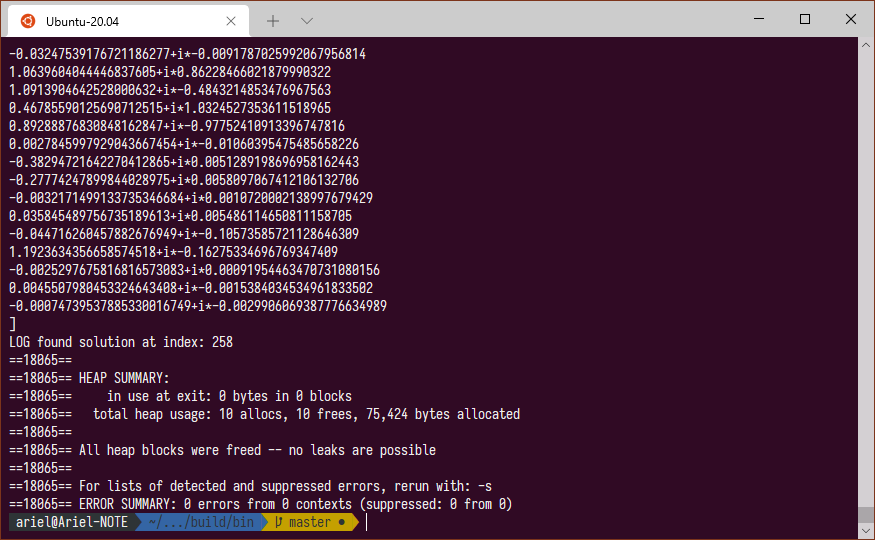
\includegraphics[width=\columnwidth]{figs/valgrind_memcheck}
    \caption{Valgrind Memcheck results}
\end{figure}

Next, we used Cachegrind to check for cache access, cache misses and branch
mispredictions, of which both were under 4\%.

\begin{figure}[H]
    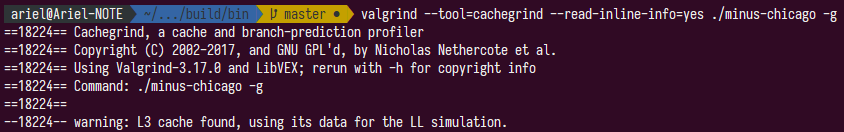
\includegraphics[width=\columnwidth]{figs/valgrind_cachegrind}
    \caption{Valgrind Cachegrind}
\end{figure}
\begin{figure}[H]
    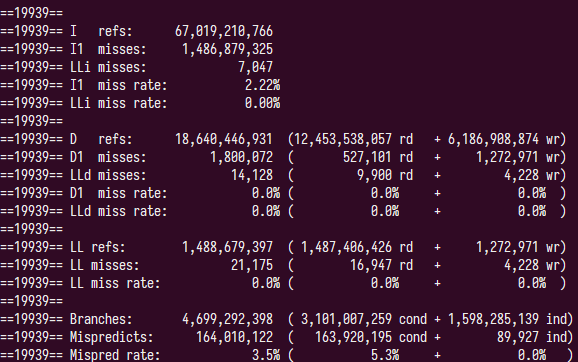
\includegraphics[width=\columnwidth]{figs/valgrind_cachegrind_results}
    \caption{Valgrind Cachegrind results}
\end{figure}

The tool Gg\_annotate allows for deeper understanding of the cache access
patterns which can be used to optimize memory access within functions.

\begin{figure}[H]
    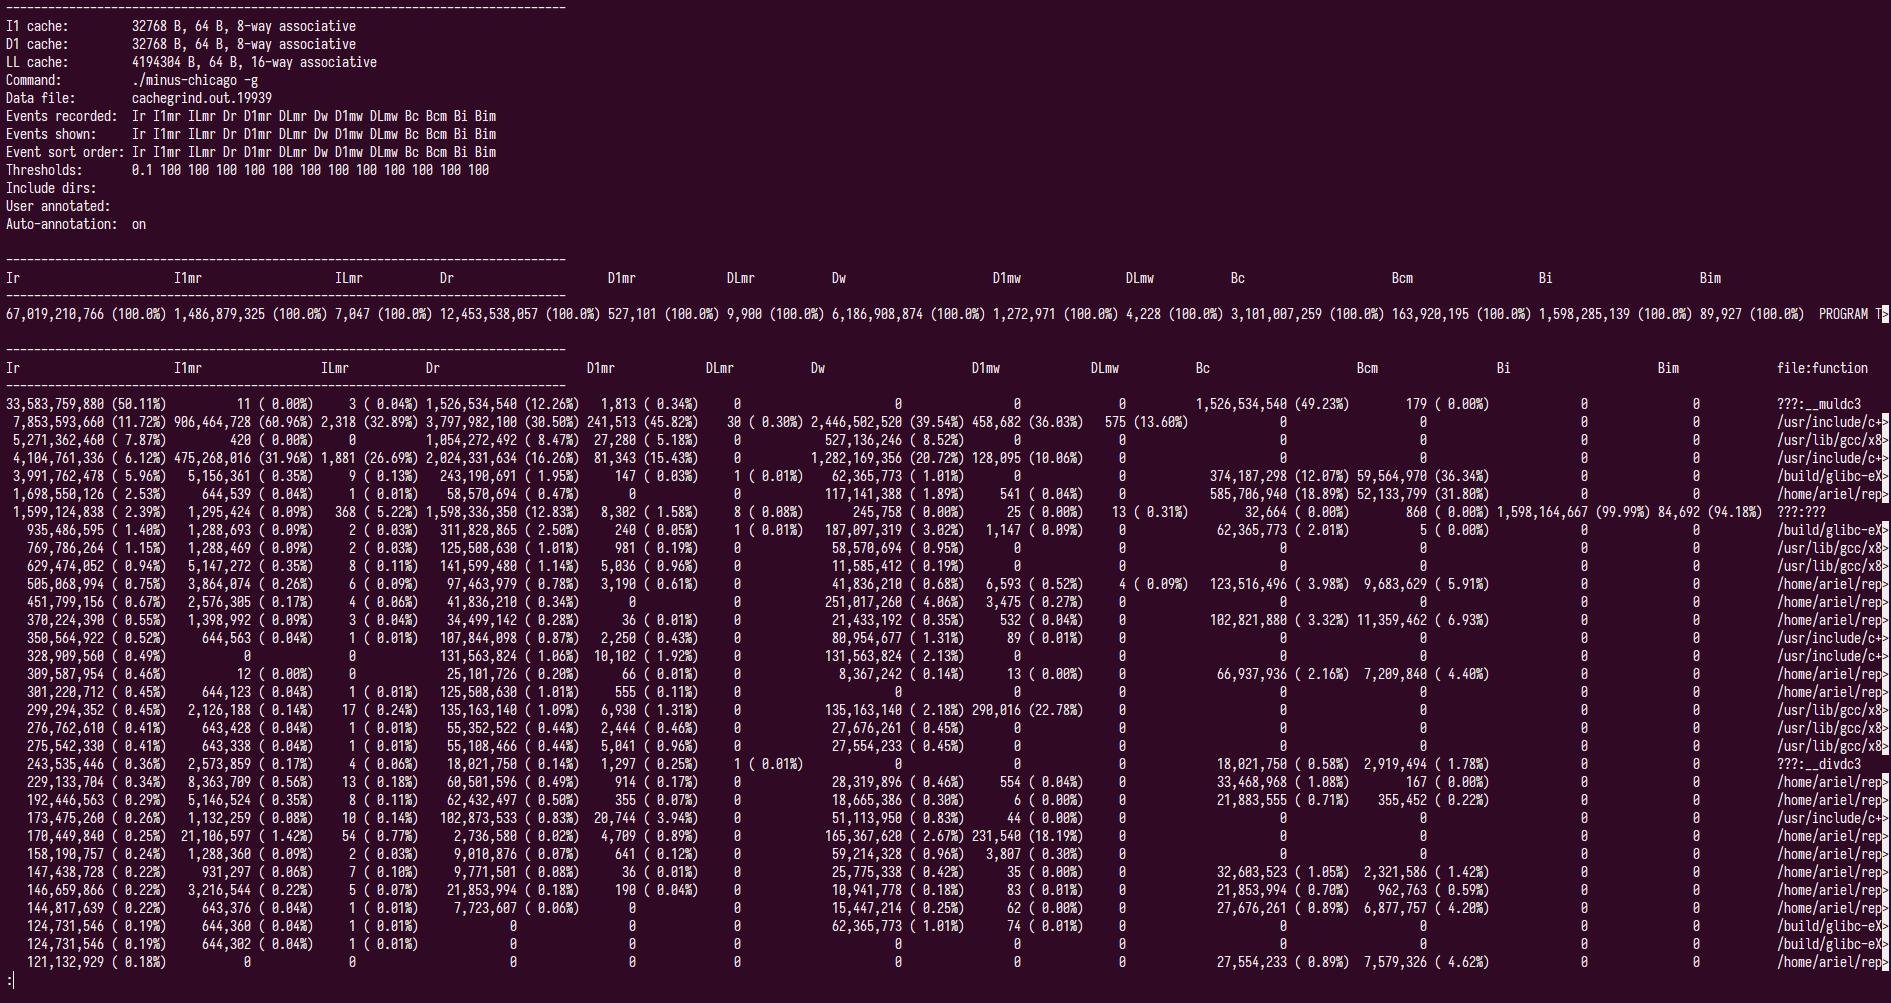
\includegraphics[width=\columnwidth]{figs/valgrind_cg_annotate0}
    \caption{Valgrind Cg\_annotate (Cachegrind\_annotate) 0}
\end{figure}
\begin{figure}[H]
    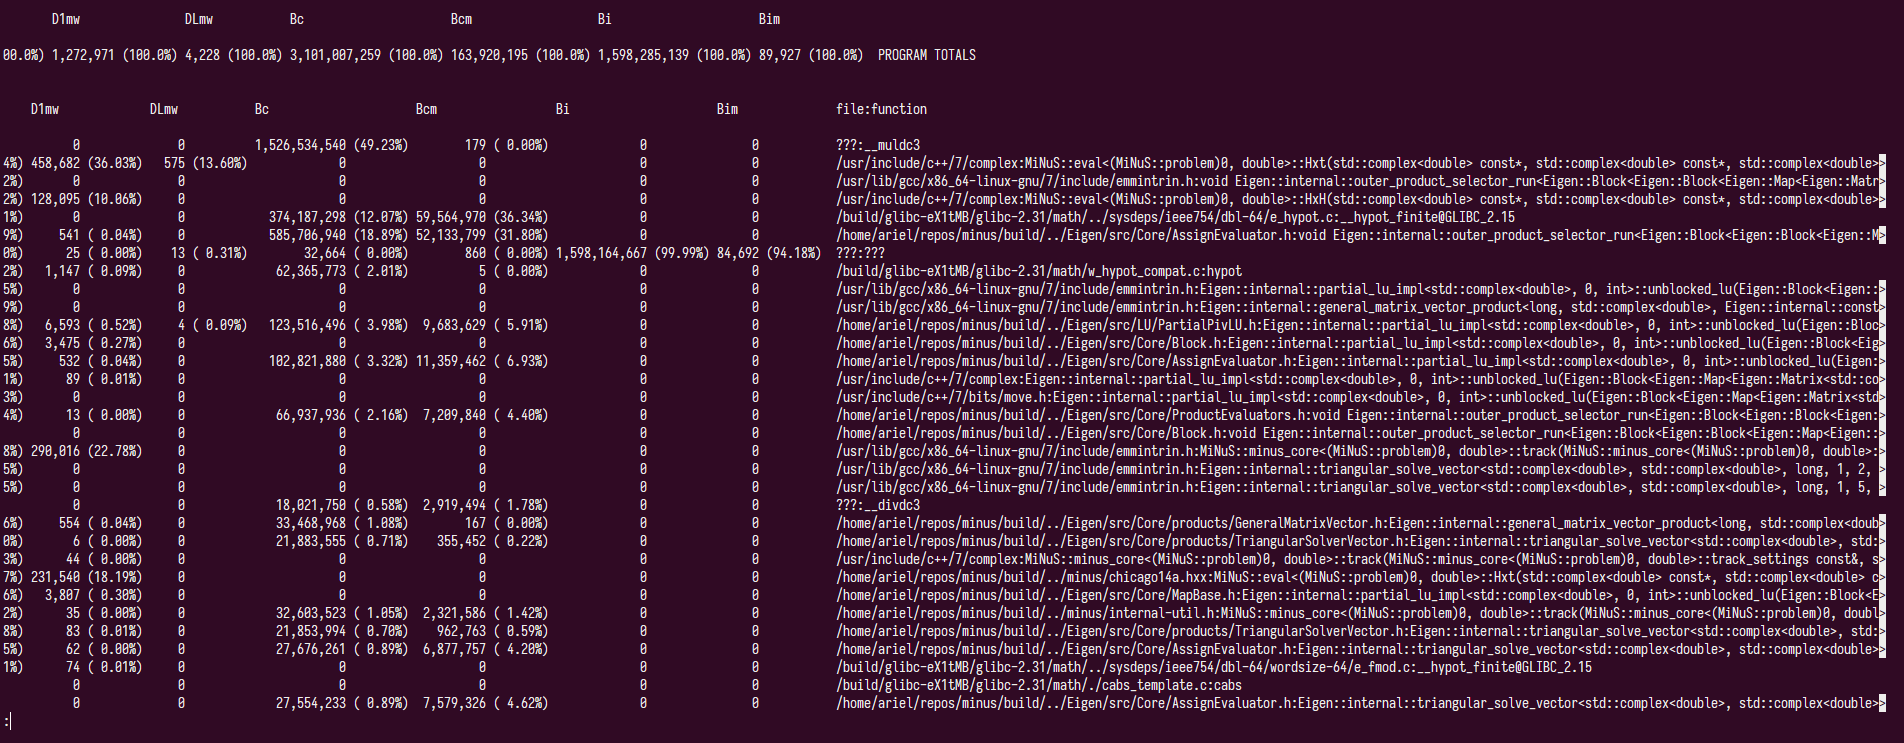
\includegraphics[width=\columnwidth]{figs/valgrind_cg_annotate1}
    \caption{Valgrind Cg\_annotate (Cachegrind\_annotate) 1}
\end{figure}

Using Callgrind in conjunction with the graphical tool QCachegrind, we can
see the function callers and callees, and what percentage of the total runtime
each one took. From this analysis, we can find that the most used function is
the GCC's library built-in complex multiplication routine, followed by the Eigen
library internal functions.

\begin{figure}[H]
    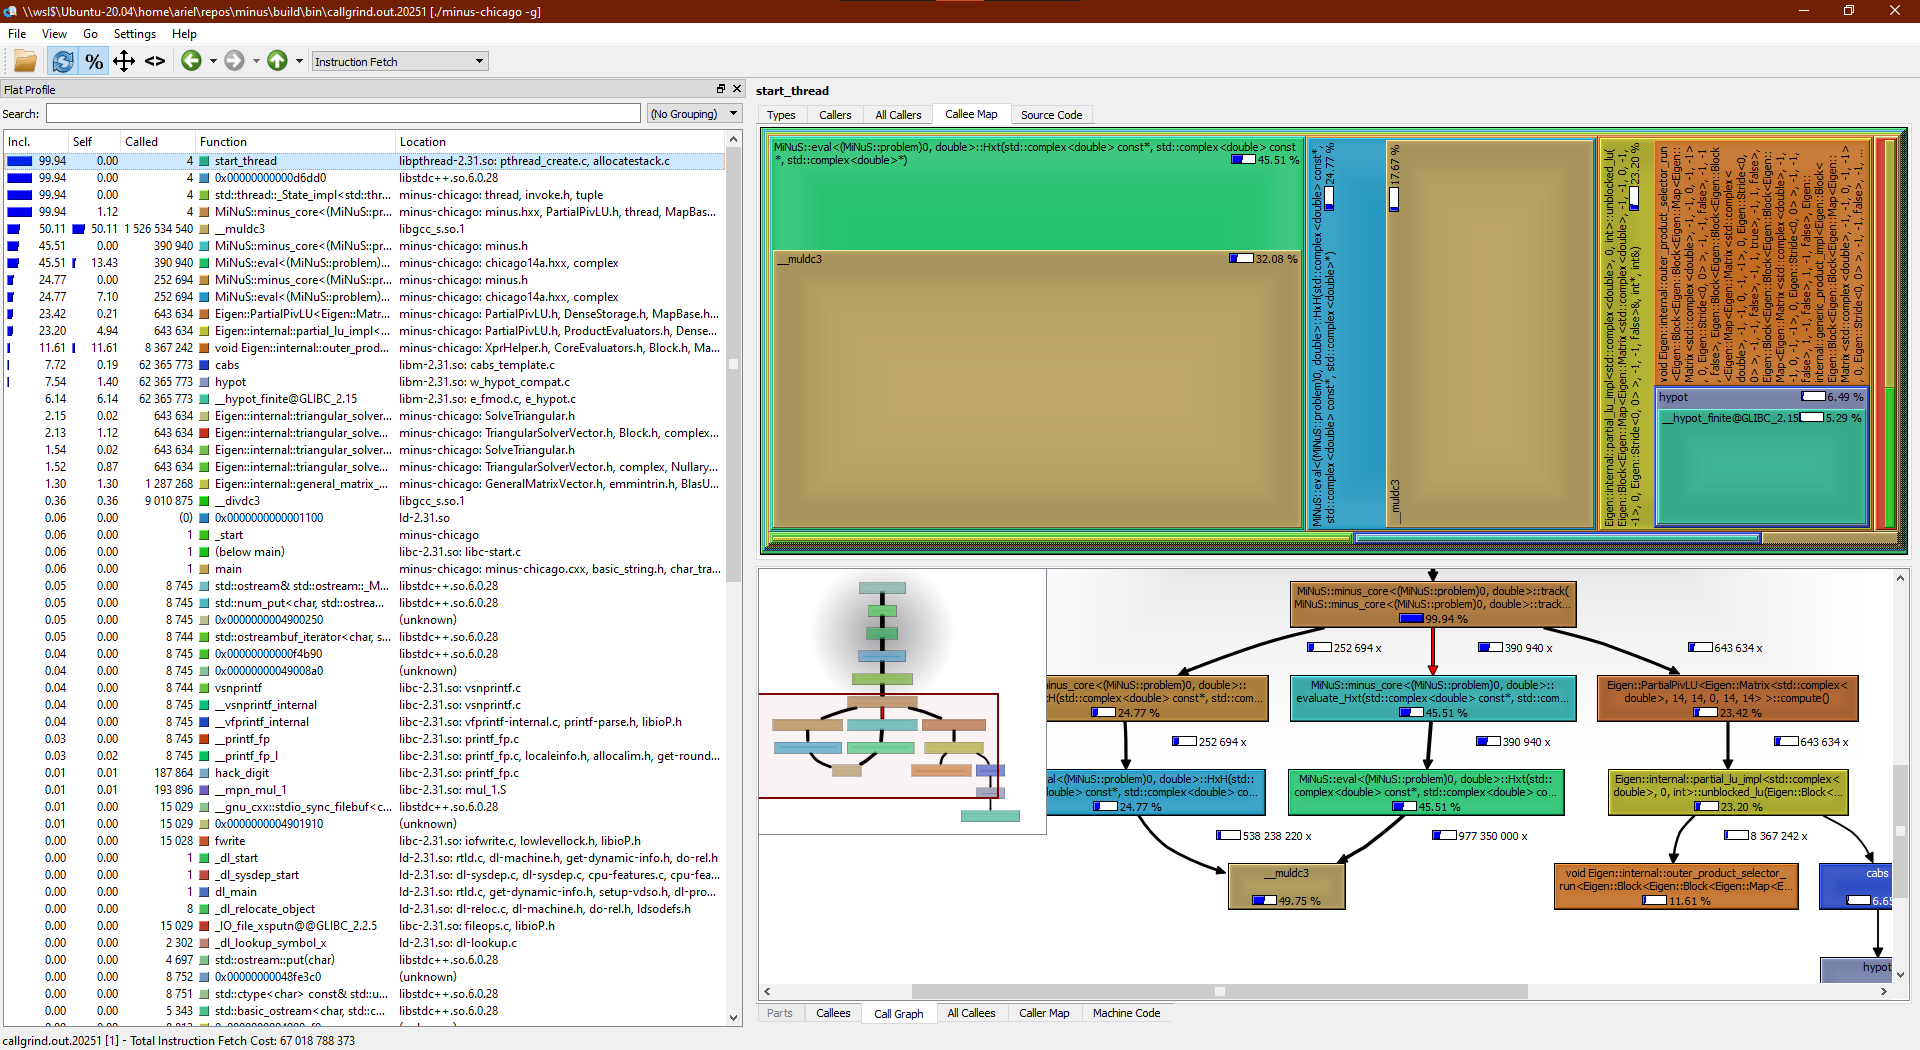
\includegraphics[width=\columnwidth]{figs/valgrind_qcachegrind_callgrind}
    \caption{Valgrind QCachegrind with Callgrind's output}
\end{figure}


\subsection{Graphical Analysis}

By tapping into the value of an element of each array we can try to detect
patterns which can be used to speedup certain calculations. For each iteration
of the main loop, we get a new value which is saved onto a text file. The lines
of this text file were loaded as an array of points in the online graphing tool
Desmos for graphical analysis.

Hxt[0]:
\begin{figure}[H]
    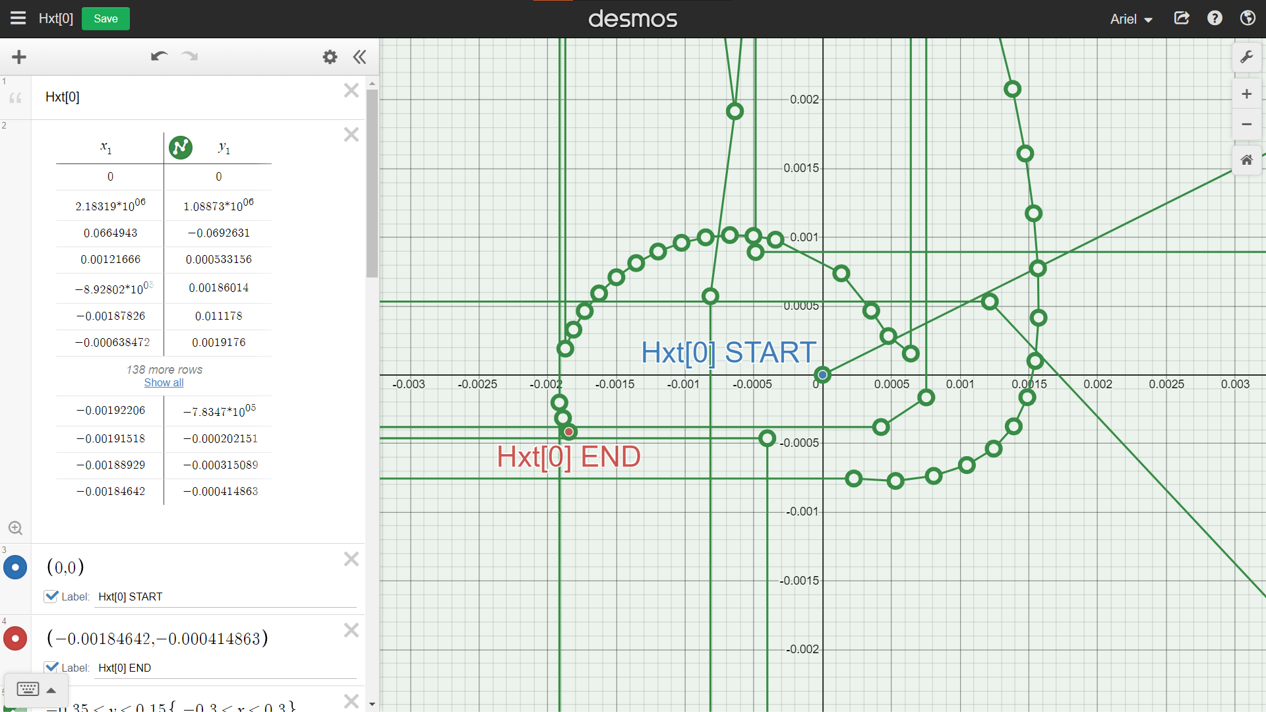
\includegraphics[width=\columnwidth]{figs/Hxt[0]_0}
    \caption{Hxt[0] 0}
\end{figure}
\begin{figure}[H]
    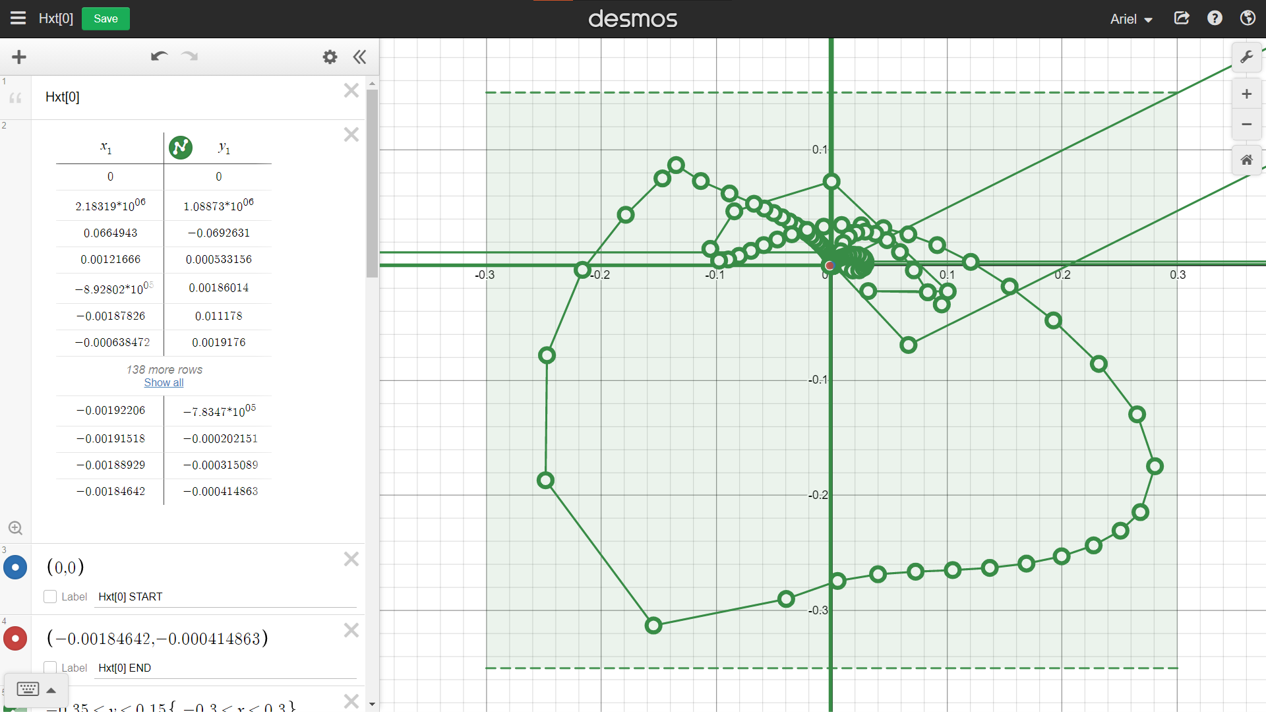
\includegraphics[width=\columnwidth]{figs/Hxt[0]_1}
    \caption{Hxt[0] 1}
\end{figure}
\begin{figure}[H]
    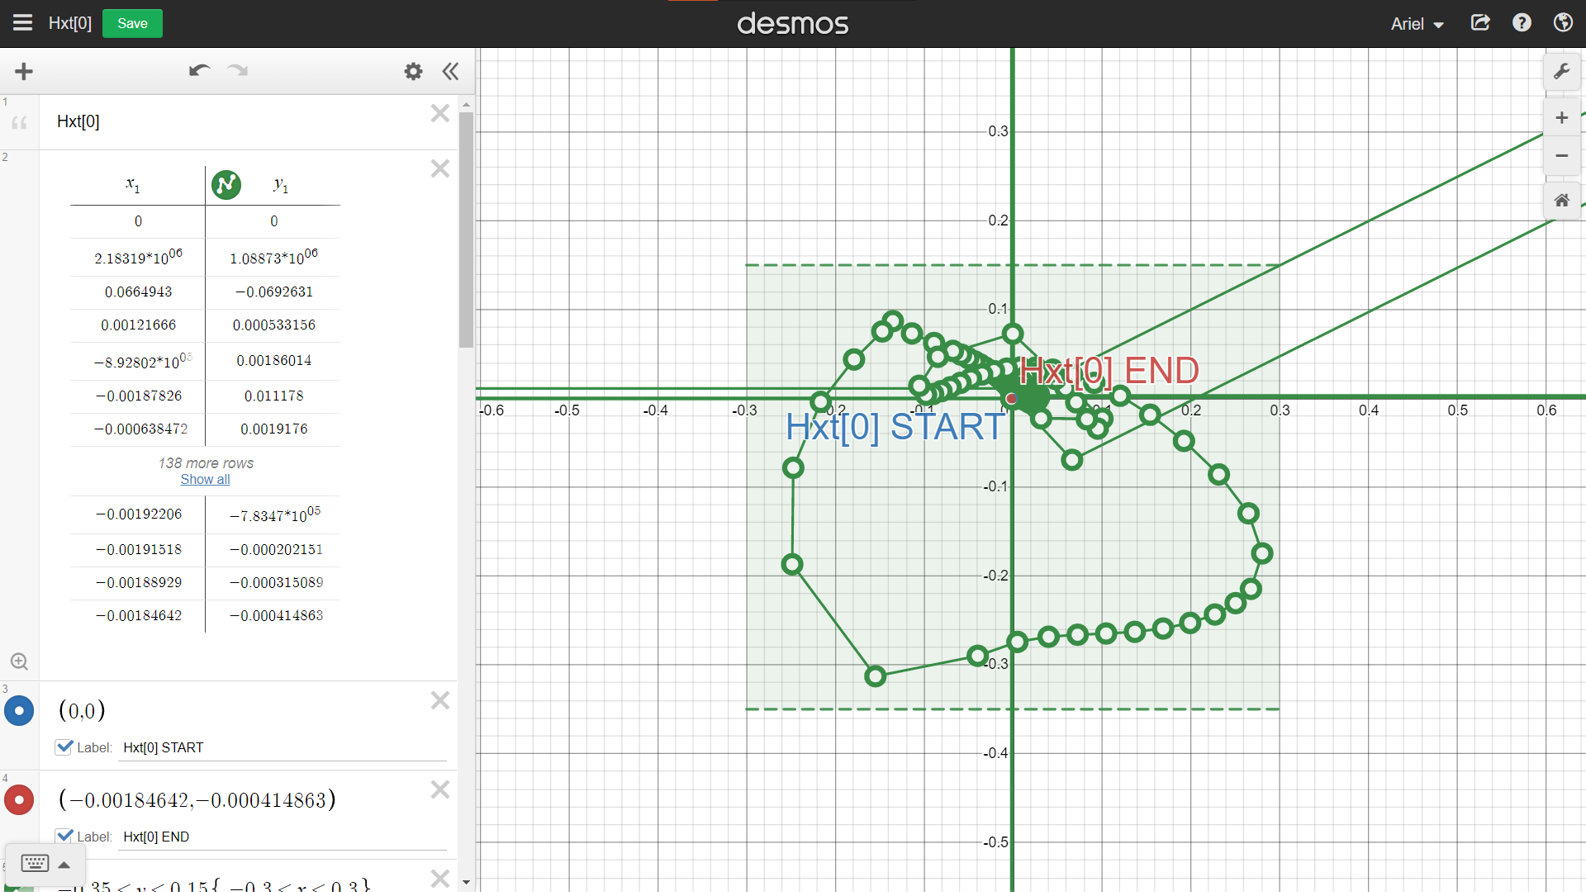
\includegraphics[width=\columnwidth]{figs/Hxt[0]_2}
    \caption{Hxt[0] 2}
\end{figure}
\begin{figure}[H]
    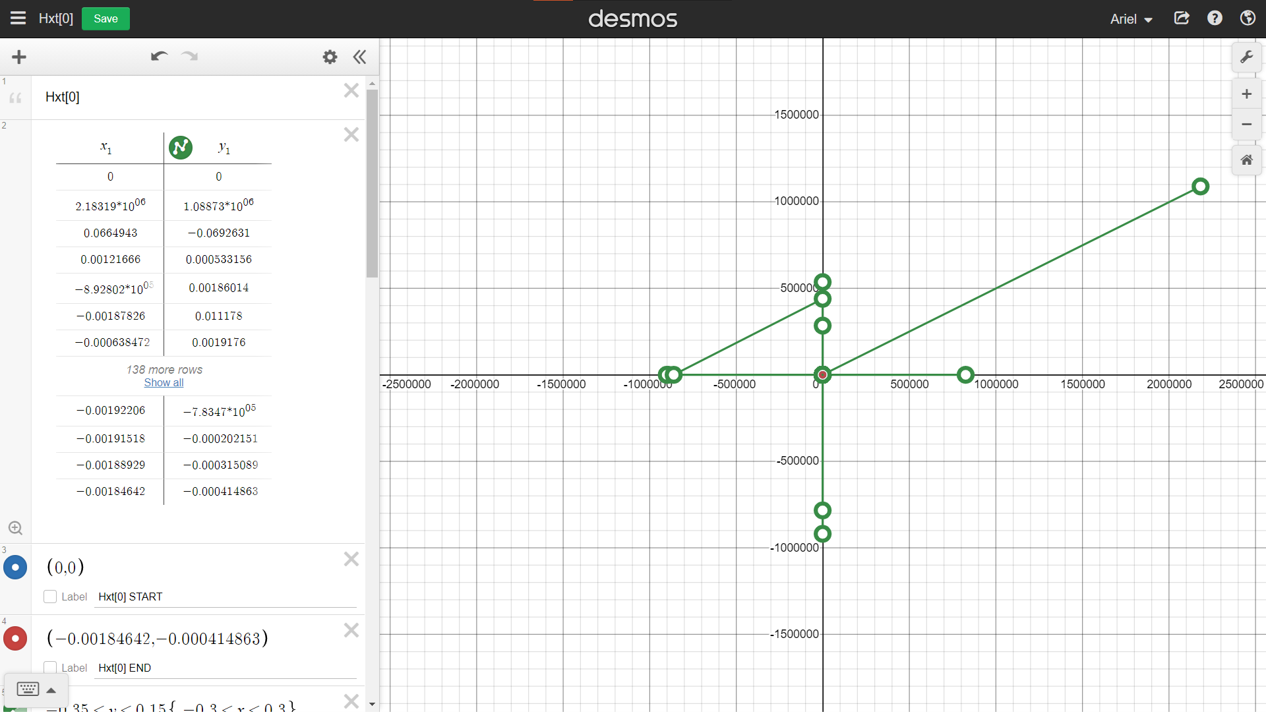
\includegraphics[width=\columnwidth]{figs/Hxt[0]_3}
    \caption{Hxt[0] 3}
\end{figure}
\begin{figure}[H]
    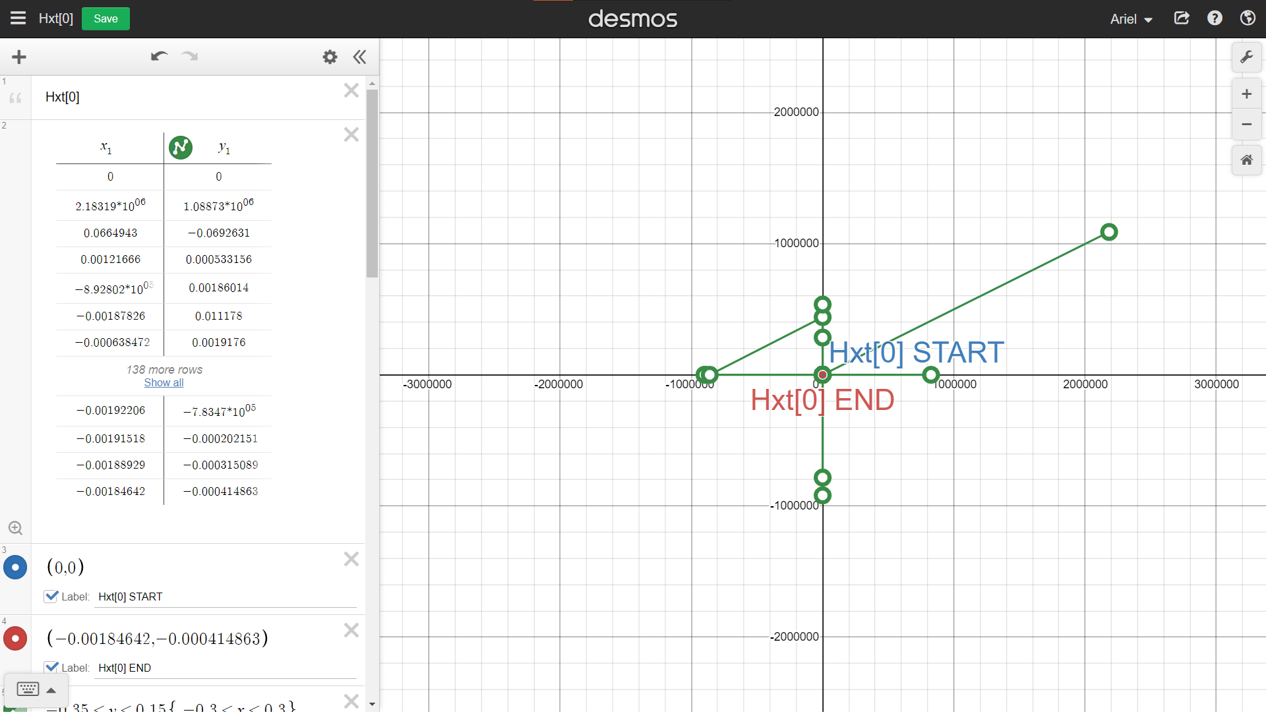
\includegraphics[width=\columnwidth]{figs/Hxt[0]_4}
    \caption{Hxt[0] 4}
\end{figure}

dxdi[0]:
\begin{figure}[H]
    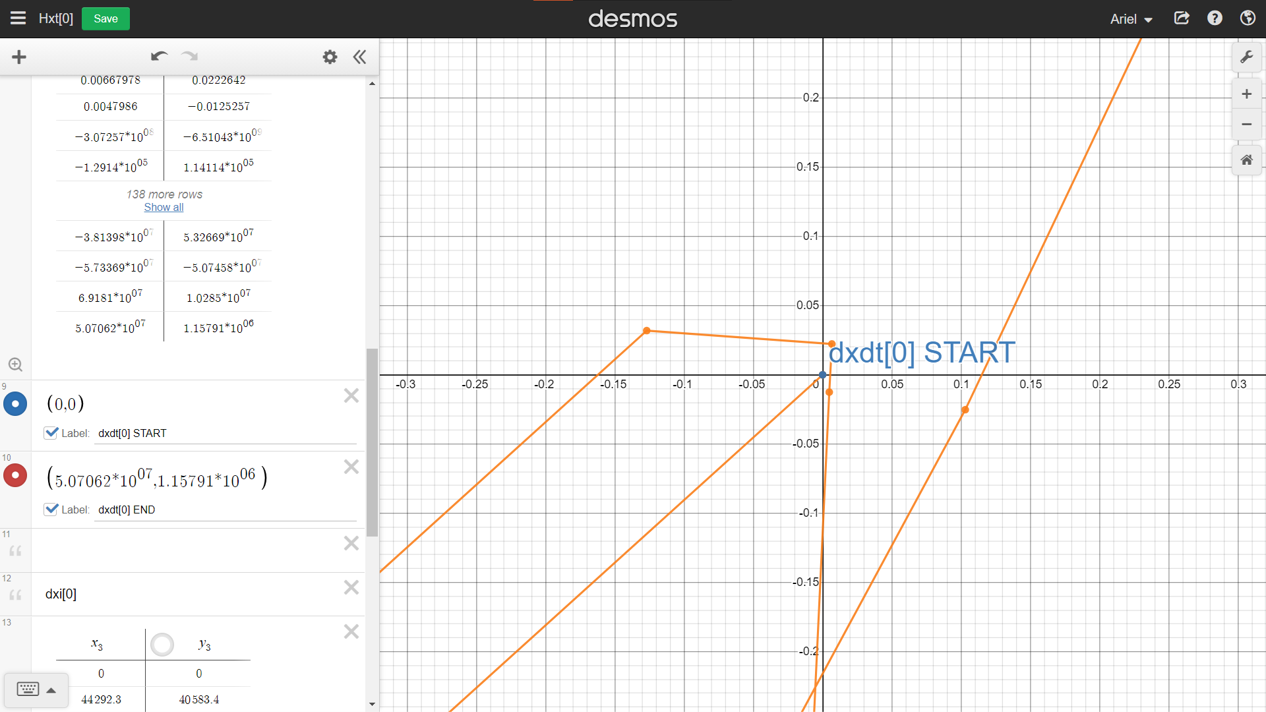
\includegraphics[width=\columnwidth]{figs/dxdi[0]_0}
    \caption{dxdi[0] 0}
\end{figure}
\begin{figure}[H]
    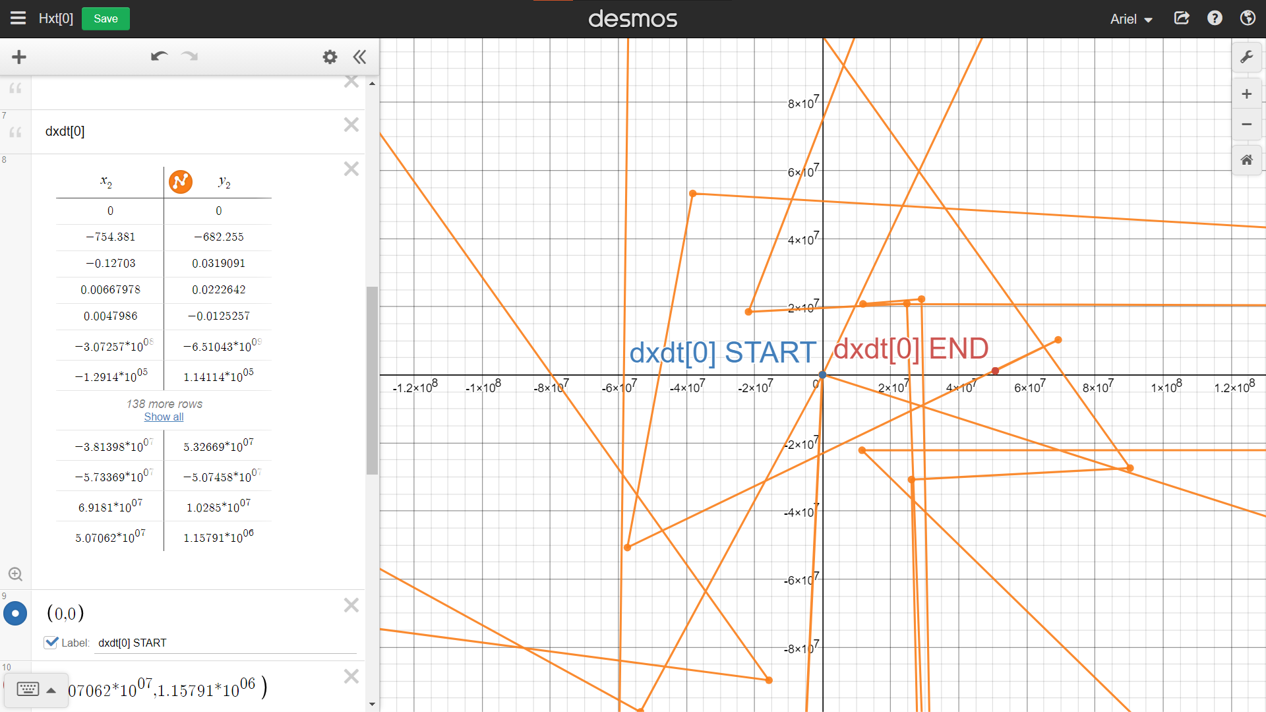
\includegraphics[width=\columnwidth]{figs/dxdi[0]_1}
    \caption{dxdi[0] 1}
\end{figure}
\begin{figure}[H]
    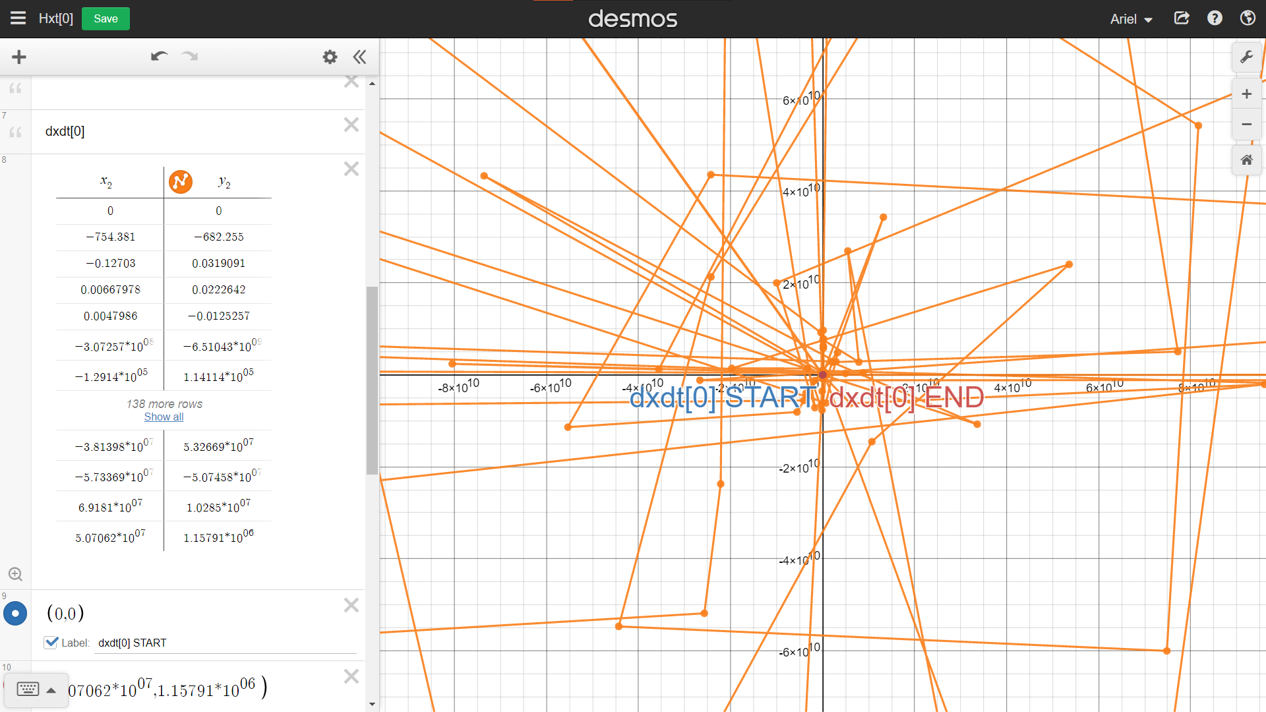
\includegraphics[width=\columnwidth]{figs/dxdi[0]_2}
    \caption{dxdi[0] 2}
\end{figure}
\begin{figure}[H]
    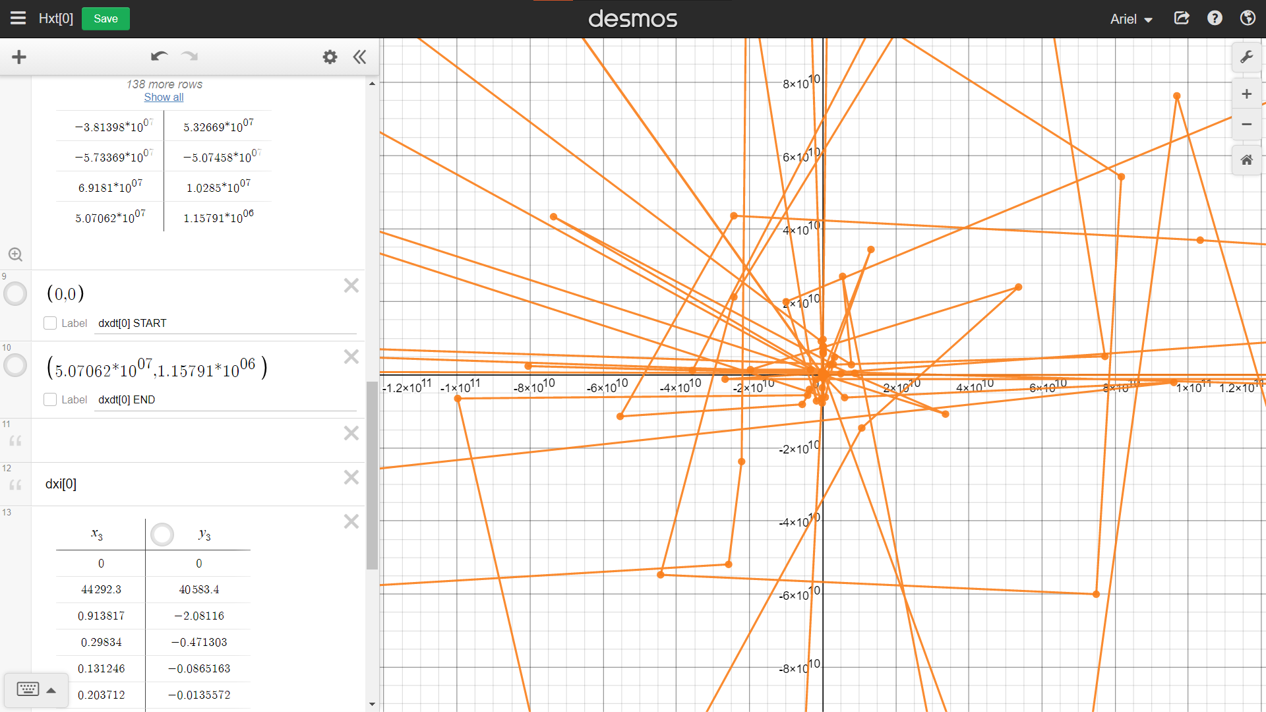
\includegraphics[width=\columnwidth]{figs/dxdi[0]_3}
    \caption{dxdi[0] 3}
\end{figure}
\begin{figure}[H]
    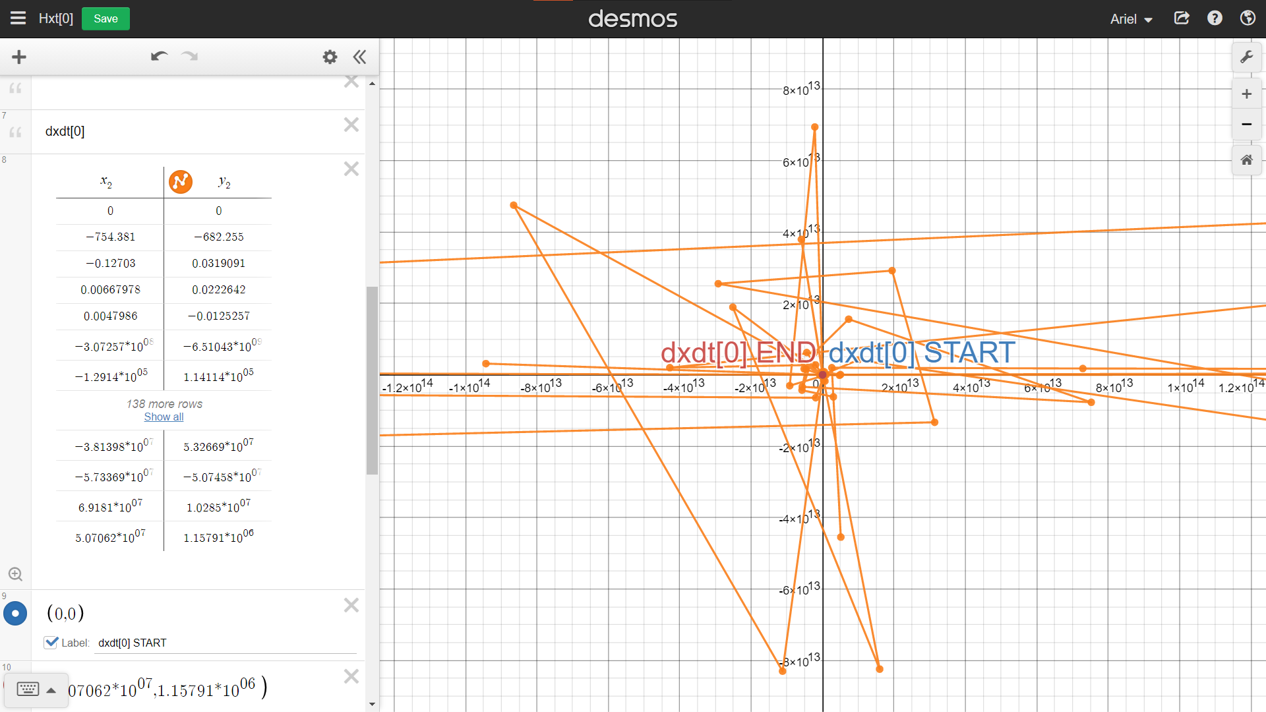
\includegraphics[width=\columnwidth]{figs/dxdi[0]_4}
    \caption{dxdi[0] 4}
\end{figure}
\begin{figure}[H]
    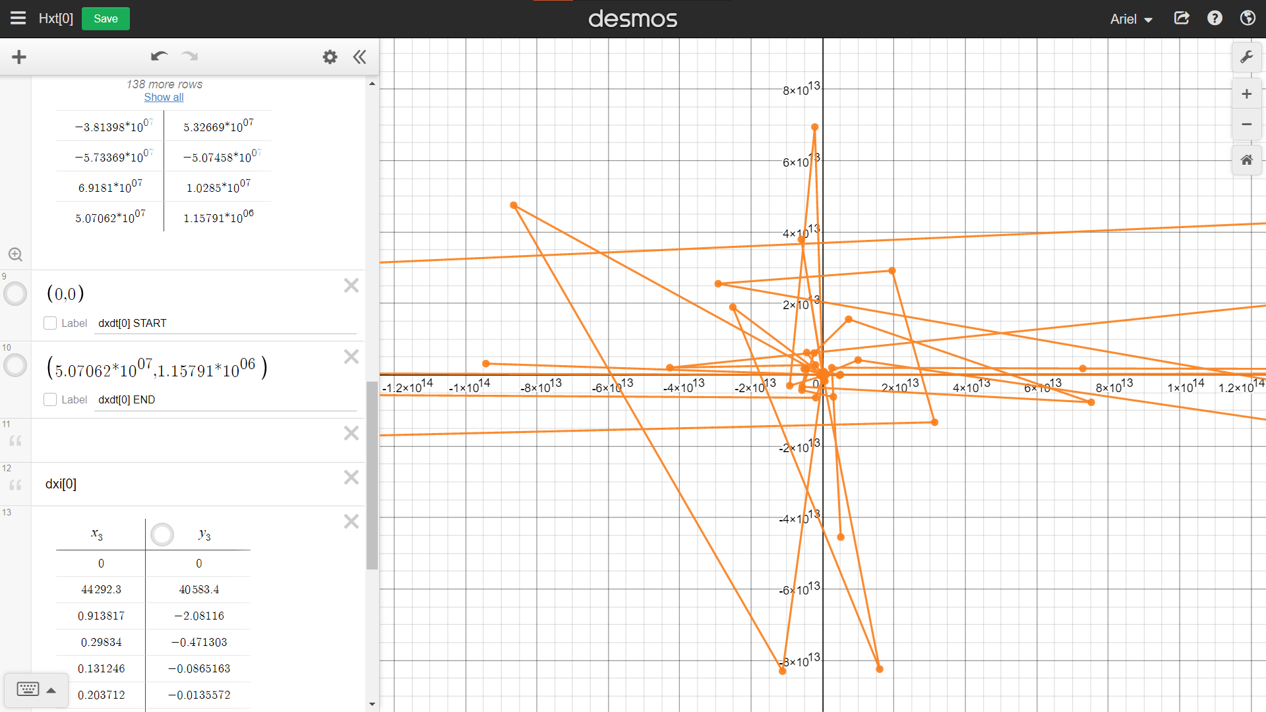
\includegraphics[width=\columnwidth]{figs/dxdi[0]_5}
    \caption{dxdi[0] 5}
\end{figure}
\begin{figure}[H]
    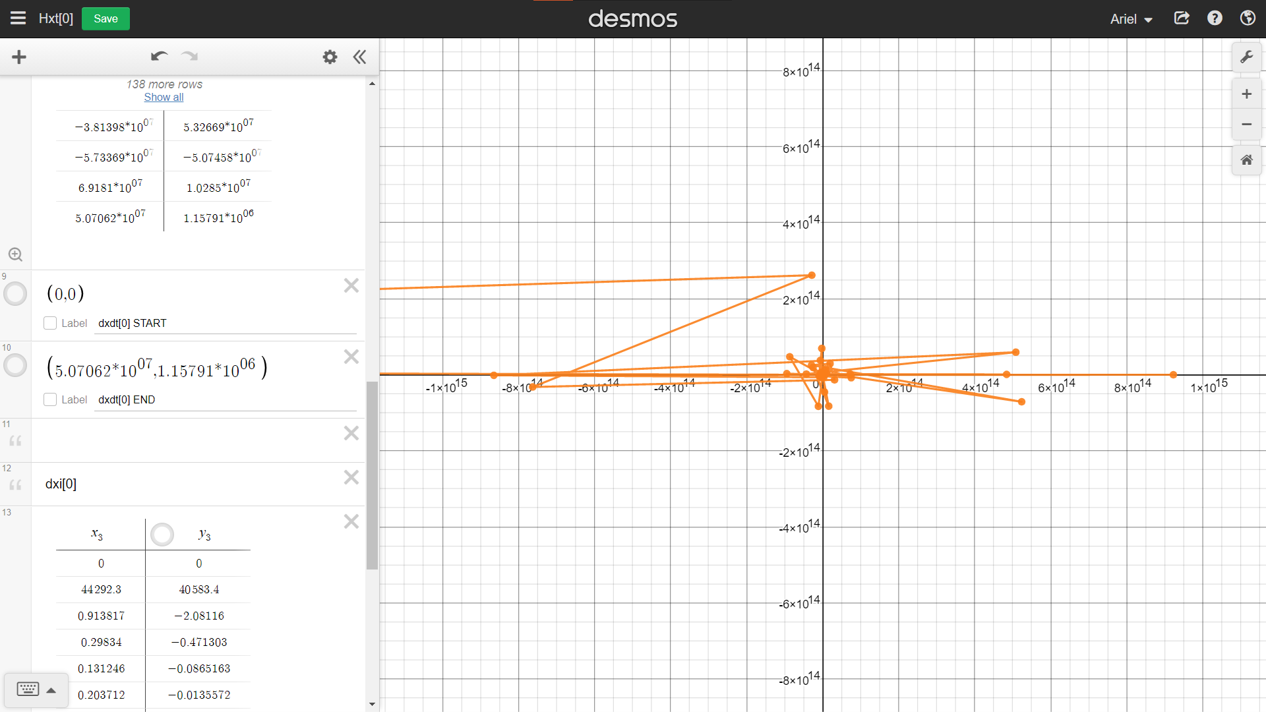
\includegraphics[width=\columnwidth]{figs/dxdi[0]_6}
    \caption{dxdi[0] 6}
\end{figure}
\begin{figure}[H]
    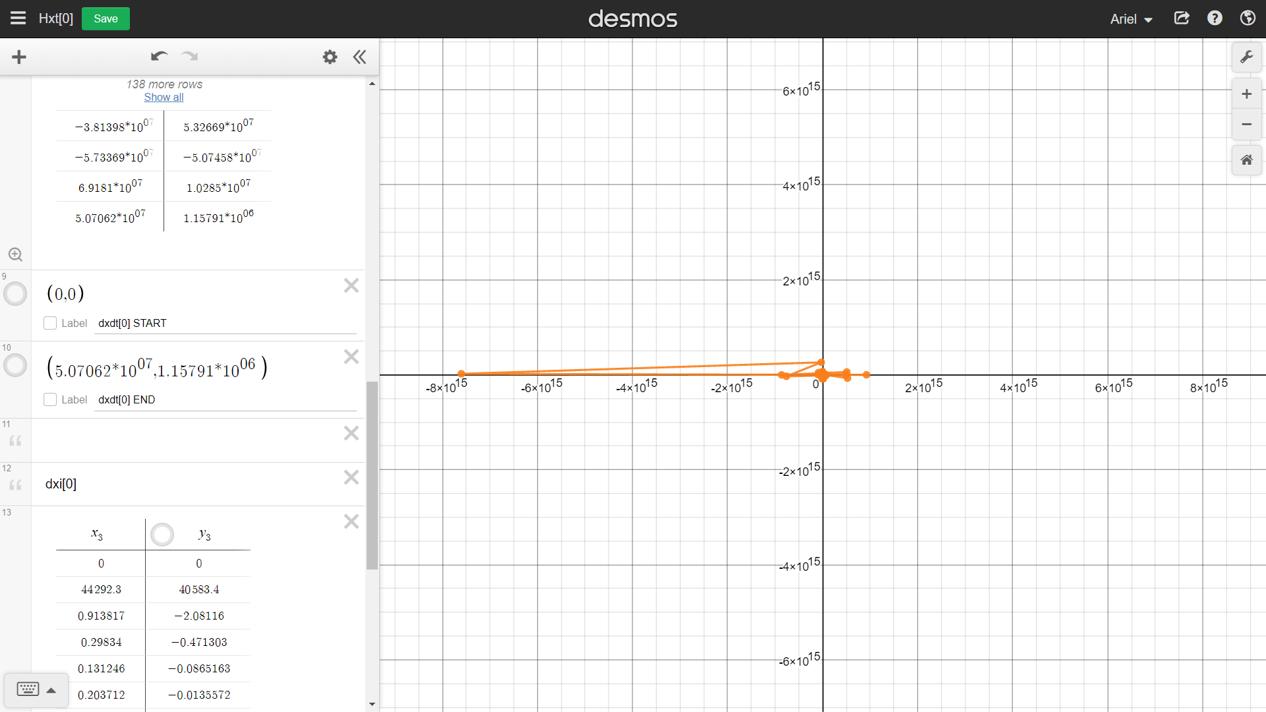
\includegraphics[width=\columnwidth]{figs/dxdi[0]_7}
    \caption{dxdi[0] 7}
\end{figure}

dxi[0]:
\begin{figure}[H]
    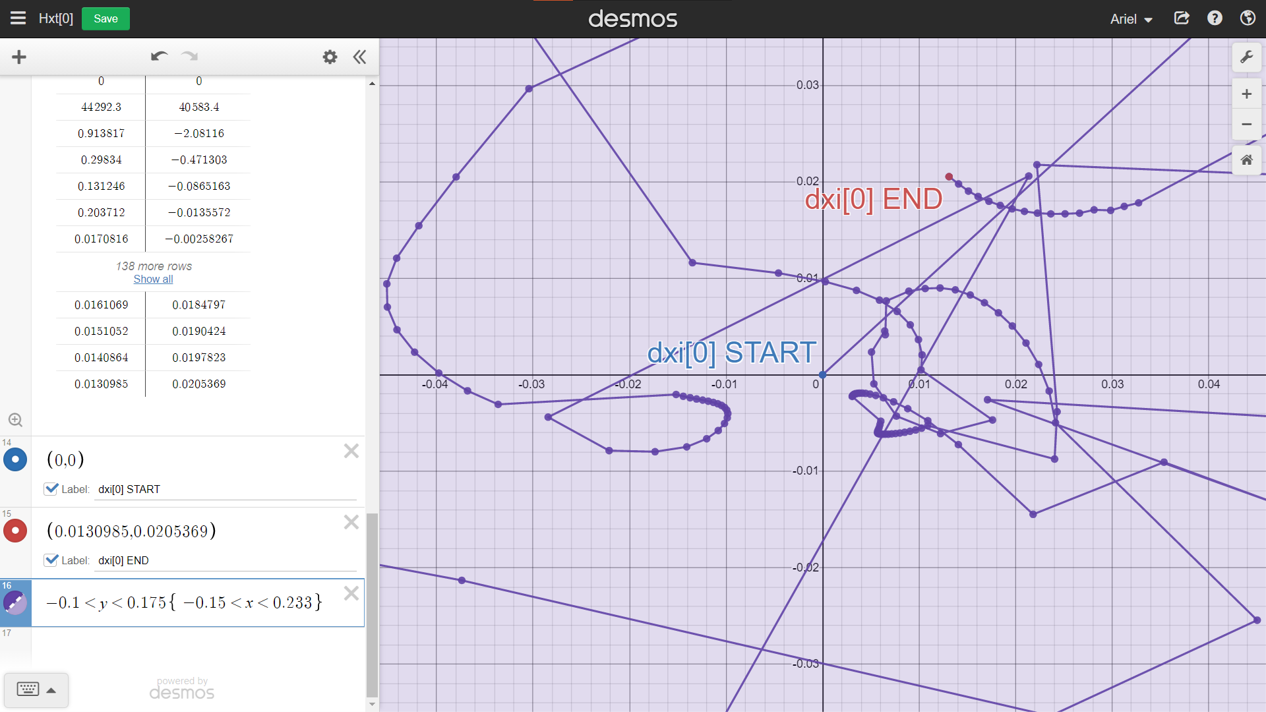
\includegraphics[width=\columnwidth]{figs/dxi[0]_0}
    \caption{dxi[0] 0}
\end{figure}
\begin{figure}[H]
    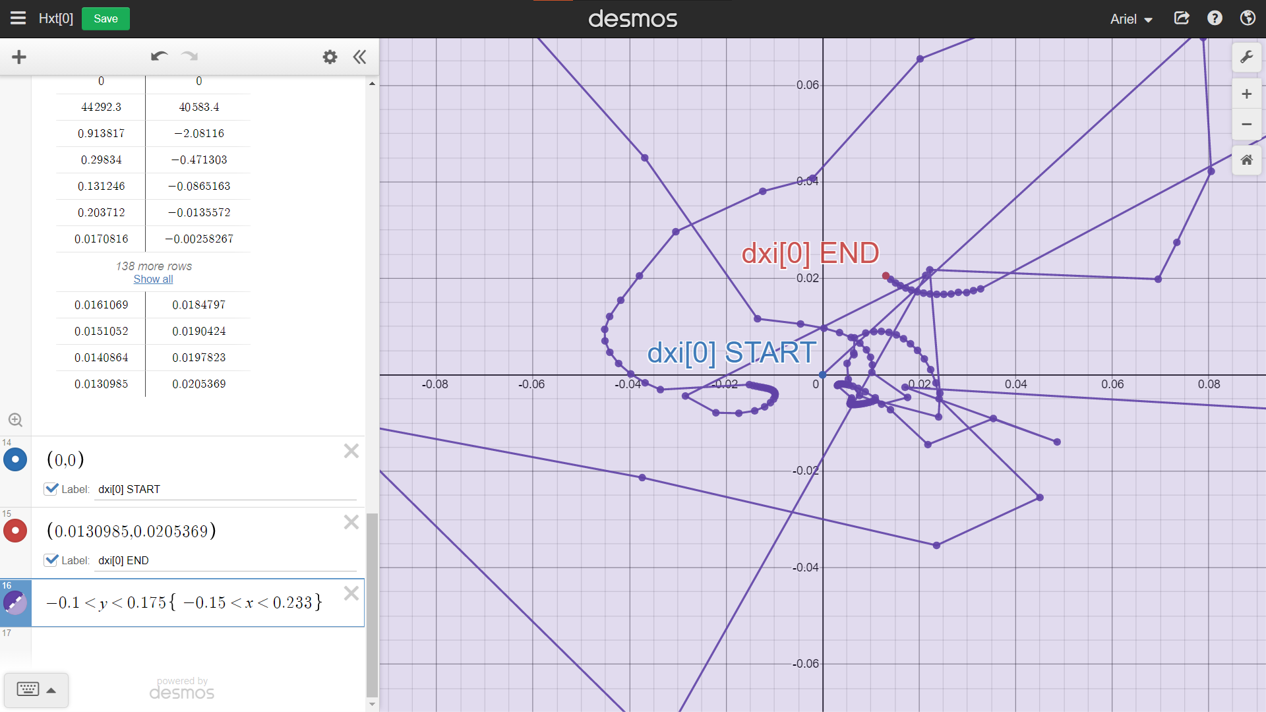
\includegraphics[width=\columnwidth]{figs/dxi[0]_1}
    \caption{dxi[0] 1}
\end{figure}
\begin{figure}[H]
    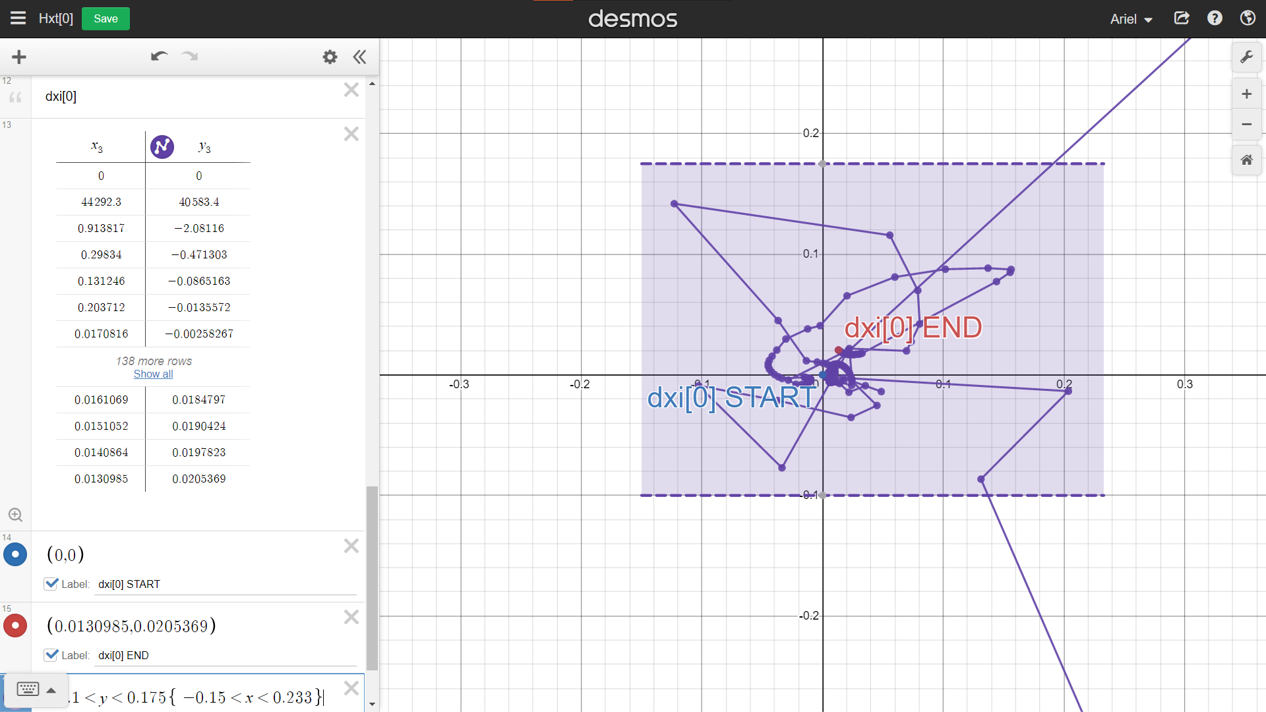
\includegraphics[width=\columnwidth]{figs/dxi[0]_2}
    \caption{dxi[0] 2}
\end{figure}
\begin{figure}[H]
    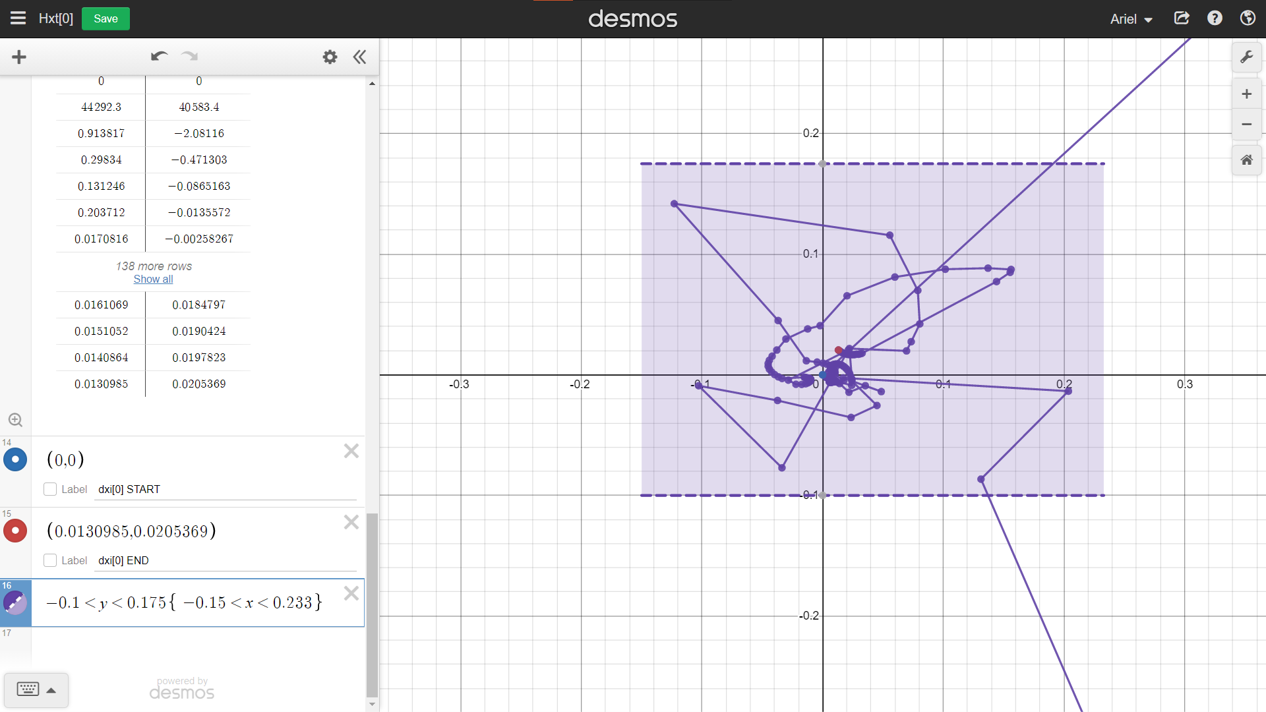
\includegraphics[width=\columnwidth]{figs/dxi[0]_3}
    \caption{dxi[0] 3}
\end{figure}
\begin{figure}[H]
    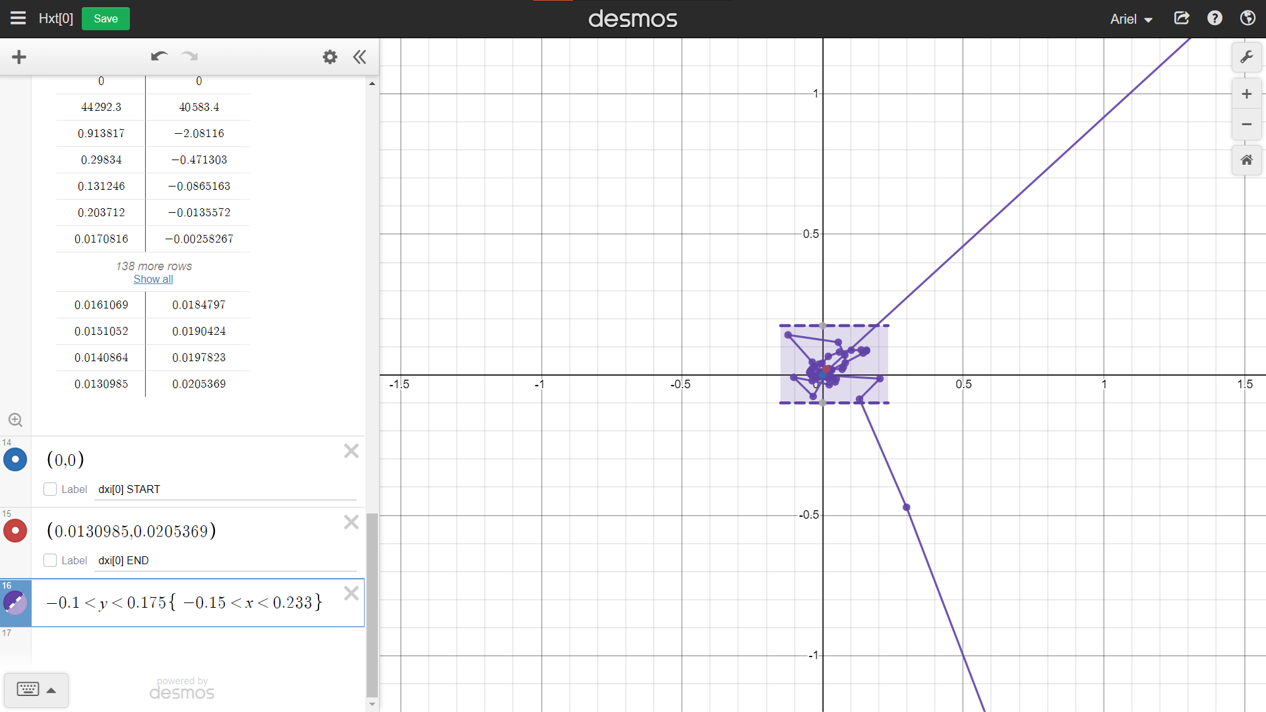
\includegraphics[width=\columnwidth]{figs/dxi[0]_4}
    \caption{dxi[0] 4}
\end{figure}
\begin{figure}[H]
    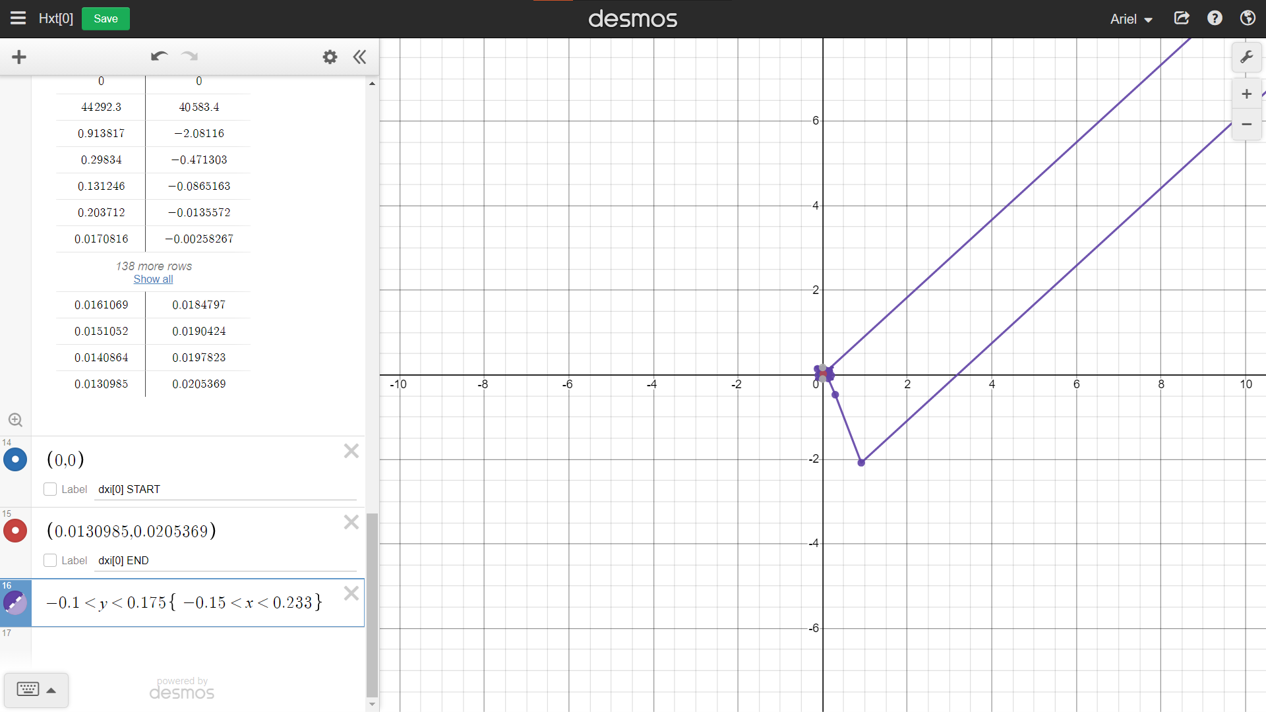
\includegraphics[width=\columnwidth]{figs/dxi[0]_5}
    \caption{dxi[0] 5}
\end{figure}
\begin{figure}[H]
    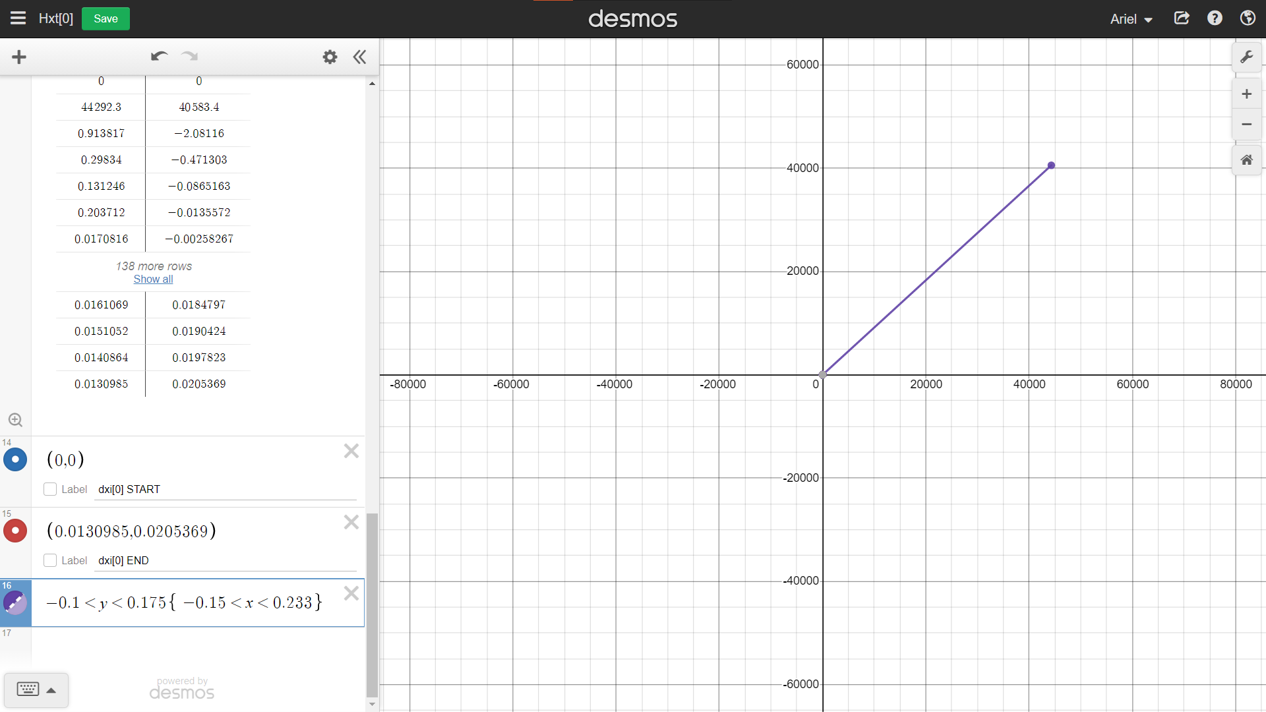
\includegraphics[width=\columnwidth]{figs/dxi[0]_6}
    \caption{dxi[0] 6}
\end{figure}


\subsection{Benchmarking Changes}
By allocating a single memory block and manually assigning pointers to specific
positions, we can eliminate the memory gap created by the compiler. Furthermore,
by using the special keyword \verb|__restrict__|, it's possible for the compiler
to optimize the code more thoroughly, as we promise it we won't cause any
pointer aliasing.

We benchmarked the program before and after the changes, and noticed a small
speedup. This may be due to fewer cache misses, as the most frequently accessed
memory segment is smaller in size.

Benchmark results:

Benchmark 20 tries before change
\footnotesize\begin{verbatim}
        Running test 1/20: 1.78s
        Running test 2/20: 1.47s
        Running test 3/20: 1.81s
        Running test 4/20: 1.52s
        Running test 5/20: 1.75s
        Running test 6/20: 1.51s
        Running test 7/20: 1.48s
        Running test 8/20: 1.42s
        Running test 9/20: 1.40s
        Running test 10/20: 1.50s
        Running test 11/20: 1.54s
        Running test 12/20: 1.44s
        Running test 13/20: 1.46s
        Running test 14/20: 1.45s
        Running test 15/20: 1.41s
        Running test 16/20: 1.48s
        Running test 17/20: 1.70s
        Running test 18/20: 1.65s
        Running test 19/20: 1.72s
        Running test 20/20: 1.81s
        AVERAGE TIME (20 RUNS): 1.56s
\end{verbatim}
\normalsize

Benchmark 20 tries after change:
\footnotesize\begin{verbatim}
    Running test 1/20: 1.54s
    Running test 2/20: 1.40s
    Running test 3/20: 1.42s
    Running test 4/20: 1.39s
    Running test 5/20: 1.40s
    Running test 6/20: 1.40s
    Running test 7/20: 1.45s
    Running test 8/20: 1.37s
    Running test 9/20: 1.38s
    Running test 10/20: 1.42s
    Running test 11/20: 1.38s
    Running test 12/20: 1.41s
    Running test 13/20: 1.37s
    Running test 14/20: 1.82s
    Running test 15/20: 1.47s
    Running test 16/20: 1.85s
    Running test 17/20: 1.71s
    Running test 18/20: 1.42s
    Running test 19/20: 1.54s
    Running test 20/20: 1.65s
    AVERAGE TIME (20 RUNS): 1.49s
\end{verbatim}
\normalsize

Benchmark 20 tries after change with \verb|__restrict__|
\footnotesize\begin{verbatim}
    Running test 1/20: 1.53s
    Running test 2/20: 1.44s
    Running test 3/20: 1.41s
    Running test 4/20: 1.40s
    Running test 5/20: 1.47s
    Running test 6/20: 1.41s
    Running test 7/20: 1.41s
    Running test 8/20: 1.42s
    Running test 9/20: 1.42s
    Running test 10/20: 1.40s
    Running test 11/20: 1.38s
    Running test 12/20: 1.44s
    Running test 13/20: 1.39s
    Running test 14/20: 1.41s
    Running test 15/20: 1.98s
    Running test 16/20: 2.01s
    Running test 17/20: 1.43s
    Running test 18/20: 1.47s
    Running test 19/20: 1.81s
    Running test 20/20: 1.57s
    AVERAGE TIME (20 RUNS): 1.51s
\end{verbatim}
\normalsize

Benchmark 5 rounds 10 tries before change
\footnotesize\begin{verbatim}
    Round 1/5
        Running test 1/10: 1440ms
        Running test 2/10: 1373ms
        Running test 3/10: 1374ms
        Running test 4/10: 1451ms
        Running test 5/10: 1409ms
        Running test 6/10: 1400ms
        Running test 7/10: 1380ms
        Running test 8/10: 1401ms
        Running test 9/10: 1397ms
        Running test 10/10: 1416ms
        AVERAGE TIME (FIRST 5 RUNS): 1409.400ms
        AVERAGE TIME (10 RUNS): 1404.100ms
    Round finished. Sleeping for 10 seconds...
    Round 2/5
        Running test 1/10: 1392ms
        Running test 2/10: 1385ms
        Running test 3/10: 1411ms
        Running test 4/10: 1375ms
        Running test 5/10: 1410ms
        Running test 6/10: 1401ms
        Running test 7/10: 1387ms
        Running test 8/10: 1528ms
        Running test 9/10: 1714ms
        Running test 10/10: 1596ms
        AVERAGE TIME (FIRST 5 RUNS): 1394.600ms
        AVERAGE TIME (10 RUNS): 1459.900ms
    Round finished. Sleeping for 10 seconds...
    Round 3/5
        Running test 1/10: 1399ms
        Running test 2/10: 1376ms
        Running test 3/10: 1390ms
        Running test 4/10: 1397ms
        Running test 5/10: 1381ms
        Running test 6/10: 1405ms
        Running test 7/10: 1407ms
        Running test 8/10: 1550ms
        Running test 9/10: 1629ms
        Running test 10/10: 1656ms
        AVERAGE TIME (FIRST 5 RUNS): 1388.600ms
        AVERAGE TIME (10 RUNS): 1459.000ms
    Round finished. Sleeping for 10 seconds...
    Round 4/5
        Running test 1/10: 1402ms
        Running test 2/10: 1394ms
        Running test 3/10: 1398ms
        Running test 4/10: 1416ms
        Running test 5/10: 1421ms
        Running test 6/10: 1413ms
        Running test 7/10: 1435ms
        Running test 8/10: 1529ms
        Running test 9/10: 1649ms
        Running test 10/10: 1639ms
        AVERAGE TIME (FIRST 5 RUNS): 1406.200ms
        AVERAGE TIME (10 RUNS): 1469.600ms
    Round finished. Sleeping for 10 seconds...
    Round 5/5
        Running test 1/10: 1403ms
        Running test 2/10: 1408ms
        Running test 3/10: 1384ms
        Running test 4/10: 1368ms
        Running test 5/10: 1411ms
        Running test 6/10: 1407ms
        Running test 7/10: 1408ms
        Running test 8/10: 1604ms
        Running test 9/10: 1753ms
        Running test 10/10: 1576ms
        AVERAGE TIME (FIRST 5 RUNS): 1394.800ms
        AVERAGE TIME (10 RUNS): 1472.200ms
    AVERAGE TIME (FIRST 5 RUNS OF EACH ROUND): 1432.000ms
    AVERAGE TIME (5 ROUNDS): 1452.960ms
\end{verbatim}
\normalsize

Benchmark 5 rounds 10 tries after change
\footnotesize\begin{verbatim}
    Round 1/5
        Running test 1/10: 1439ms
        Running test 2/10: 1402ms
        Running test 3/10: 1386ms
        Running test 4/10: 1387ms
        Running test 5/10: 1369ms
        Running test 6/10: 1378ms
        Running test 7/10: 1415ms
        Running test 8/10: 1378ms
        Running test 9/10: 1389ms
        Running test 10/10: 1388ms
        AVERAGE TIME (FIRST 5 RUNS): 1396.600ms
        AVERAGE TIME (10 RUNS): 1393.100ms
    Round finished. Sleeping for 10 seconds...
    Round 2/5
        Running test 1/10: 1419ms
        Running test 2/10: 1386ms
        Running test 3/10: 1406ms
        Running test 4/10: 1418ms
        Running test 5/10: 1365ms
        Running test 6/10: 1384ms
        Running test 7/10: 1373ms
        Running test 8/10: 1376ms
        Running test 9/10: 1497ms
        Running test 10/10: 1609ms
        AVERAGE TIME (FIRST 5 RUNS): 1398.800ms
        AVERAGE TIME (10 RUNS): 1423.300ms
    Round finished. Sleeping for 10 seconds...
    Round 3/5
        Running test 1/10: 1422ms
        Running test 2/10: 1557ms
        Running test 3/10: 1400ms
        Running test 4/10: 1397ms
        Running test 5/10: 1441ms
        Running test 6/10: 1376ms
        Running test 7/10: 1401ms
        Running test 8/10: 1598ms
        Running test 9/10: 1621ms
        Running test 10/10: 1618ms
        AVERAGE TIME (FIRST 5 RUNS): 1443.400ms
        AVERAGE TIME (10 RUNS): 1483.100ms
    Round finished. Sleeping for 10 seconds...
    Round 4/5
        Running test 1/10: 1414ms
        Running test 2/10: 1386ms
        Running test 3/10: 1374ms
        Running test 4/10: 1400ms
        Running test 5/10: 1381ms
        Running test 6/10: 1406ms
        Running test 7/10: 1385ms
        Running test 8/10: 1762ms
        Running test 9/10: 1511ms
        Running test 10/10: 1621ms
        AVERAGE TIME (FIRST 5 RUNS): 1391.000ms
        AVERAGE TIME (10 RUNS): 1464.000ms
    Round finished. Sleeping for 10 seconds...
    Round 5/5
        Running test 1/10: 1380ms
        Running test 2/10: 1378ms
        Running test 3/10: 1385ms
        Running test 4/10: 1372ms
        Running test 5/10: 1364ms
        Running test 6/10: 1411ms
        Running test 7/10: 1378ms
        Running test 8/10: 1737ms
        Running test 9/10: 1778ms
        Running test 10/10: 1635ms
        AVERAGE TIME (FIRST 5 RUNS): 1375.800ms
        AVERAGE TIME (10 RUNS): 1481.800ms
    AVERAGE TIME (FIRST 5 RUNS OF EACH ROUND): 1408.200ms
    AVERAGE TIME (5 ROUNDS): 1449.060ms
\end{verbatim}
\normalsize

Benchmark 5 rounds 10 tries with \verb|__restrict__|
\footnotesize\begin{verbatim}
    Round 1/5
        Running test 1/10: 1390ms
        Running test 2/10: 1369ms
        Running test 3/10: 1346ms
        Running test 4/10: 1355ms
        Running test 5/10: 1393ms
        Running test 6/10: 1391ms
        Running test 7/10: 1370ms
        Running test 8/10: 1384ms
        Running test 9/10: 1362ms
        Running test 10/10: 1420ms
        AVERAGE TIME (FIRST 5 RUNS): 1370.600ms
        AVERAGE TIME (10 RUNS): 1378.000ms
    Round finished. Sleeping for 10 seconds...
    Round 2/5
        Running test 1/10: 1370ms
        Running test 2/10: 1379ms
        Running test 3/10: 1373ms
        Running test 4/10: 1402ms
        Running test 5/10: 1364ms
        Running test 6/10: 1505ms
        Running test 7/10: 1532ms
        Running test 8/10: 1371ms
        Running test 9/10: 1404ms
        Running test 10/10: 1543ms
        AVERAGE TIME (FIRST 5 RUNS): 1377.600ms
        AVERAGE TIME (10 RUNS): 1424.300ms
    Round finished. Sleeping for 10 seconds...
    Round 3/5
        Running test 1/10: 1383ms
        Running test 2/10: 1356ms
        Running test 3/10: 1379ms
        Running test 4/10: 1368ms
        Running test 5/10: 1391ms
        Running test 6/10: 1380ms
        Running test 7/10: 1382ms
        Running test 8/10: 1438ms
        Running test 9/10: 1619ms
        Running test 10/10: 1624ms
        AVERAGE TIME (FIRST 5 RUNS): 1375.400ms
        AVERAGE TIME (10 RUNS): 1432.000ms
    Round finished. Sleeping for 10 seconds...
    Round 4/5
        Running test 1/10: 1402ms
        Running test 2/10: 1361ms
        Running test 3/10: 1358ms
        Running test 4/10: 1380ms
        Running test 5/10: 1413ms
        Running test 6/10: 1379ms
        Running test 7/10: 1396ms
        Running test 8/10: 1503ms
        Running test 9/10: 1630ms
        Running test 10/10: 1604ms
        AVERAGE TIME (FIRST 5 RUNS): 1382.800ms
        AVERAGE TIME (10 RUNS): 1442.600ms
    Round finished. Sleeping for 10 seconds...
    Round 5/5
        Running test 1/10: 1452ms
        Running test 2/10: 1479ms
        Running test 3/10: 1392ms
        Running test 4/10: 1365ms
        Running test 5/10: 1369ms
        Running test 6/10: 1422ms
        Running test 7/10: 1477ms
        Running test 8/10: 1651ms
        Running test 9/10: 1597ms
        Running test 10/10: 1617ms
        AVERAGE TIME (FIRST 5 RUNS): 1411.400ms
        AVERAGE TIME (10 RUNS): 1482.100ms
    AVERAGE TIME (FIRST 5 RUNS OF EACH ROUND): 1401.150ms
    AVERAGE TIME (5 ROUNDS): 1431.800ms
\end{verbatim}
\normalsize


% An example of a floating figure using the graphicx package.
% Note that \label must occur AFTER (or within) \caption.
% For figures, \caption should occur after the \includegraphics.
% Note that IEEEtran v1.7 and later has special internal code that
% is designed to preserve the operation of \label within \caption
% even when the captionsoff option is in effect. However, because
% of issues like this, it may be the safest practice to put all your
% \label just after \caption rather than within \caption{}.
%
% Reminder: the "draftcls" or "draftclsnofoot", not "draft", class
% option should be used if it is desired that the figures are to be
% displayed while in draft mode.
%
% \begin{figure}[!t]
% \centering
% 
\includegraphics[width=2.5in]{sibgrapi2021.png}
% where an .eps filename suffix will be assumed under latex,
% and a .pdf suffix will be assumed for pdflatex; or what has been declared
% via \DeclareGraphicsExtensions.
% \caption{SIBGRAPI - Conference on Graphics, Patterns and Images.}
% \label{fig_sim}
% \end{figure}

% Note that the IEEE typically puts floats only at the top, even when this
% results in a large percentage of a column being occupied by floats.


% An example of a double column floating figure using two subfigures.
% (The subfig.sty package must be loaded for this to work.)
% The subfigure \label commands are set within each subfloat command,
% and the \label for the overall figure must come after \caption.
% \hfil is used as a separator to get equal spacing.
% Watch out that the combined width of all the subfigures on a
% line do not exceed the text width or a line break will occur.
%
% \begin{figure*}[!t]
% \centering
% \subfloat[Case I]{
\includegraphics[width=2.5in]{figs/sibgrapi2021.png}%
% \label{fig_first_case}}
% \hfil
% \subfloat[Case II]{
\includegraphics[width=2.5in]{figs/sibgrapi2021.png}%
% \label{fig_second_case}}
% \caption{SIBGRAPI - Conference on Graphics, Patterns and Images.}
% \label{fig_sim2}
% \end{figure*}
%
% Note that often IEEE papers with subfigures do not employ subfigure
% captions (using the optional argument to \subfloat[]), but instead will
% reference/describe all of them (a), (b), etc., within the main caption.
% Be aware that for subfig.sty to generate the (a), (b), etc., subfigure
% labels, the optional argument to \subfloat must be present. If a
% subcaption is not desired, just leave its contents blank,
% e.g., \subfloat[].


% An example of a floating table. Note that, for IEEE style tables, the
% \caption command should come BEFORE the table and, given that table
% captions serve much like titles, are usually capitalized except for words
% such as a, an, and, as, at, but, by, for, in, nor, of, on, or, the, to
% and up, which are usually not capitalized unless they are the first or
% last word of the caption. Table text will default to \footnotesize as
% the IEEE normally uses this smaller font for tables.
% The \label must come after \caption as always.
%
% \begin{table}[tbp]
%% increase table row spacing, adjust to taste
% \renewcommand{\arraystretch}{1.3}
% if using array.sty, it might be a good idea to tweak the value of
% \extrarowheight as needed to properly center the text within the cells
% \caption{An Example of a Table}
% \label{table_example}
% \centering
%% Some packages, such as MDW tools, offer better commands for making tables
%% than the plain LaTeX2e tabular which is used here.
% \begin{tabular}{|c||c|}
% \hline
% One & Two\\
% \hline
% Three & Four\\
% \hline
% \end{tabular}
% \end{table}


% Note that the IEEE does not put floats in the very first column
% - or typically anywhere on the first page for that matter. Also,
% in-text middle ("here") positioning is typically not used, but it
% is allowed and encouraged for Computer Society conferences (but
% not Computer Society journals). Most IEEE journals/conferences use
% top floats exclusively.
% Note that, LaTeX2e, unlike IEEE journals/conferences, places
% footnotes above bottom floats. This can be corrected via the
% \fnbelowfloat command of the stfloats package.




\section{Conclusion}
The techniques are
useful for similar algorithms such as simulating nonrigid deformation and
dynamical systems.




% conference papers do not normally have an appendix


% use section* for acknowledgment
\section*{Acknowledgment}


The authors would like to thank...


% trigger a \newpage just before the given reference
% number - used to balance the columns on the last page
% adjust value as needed - may need to be readjusted if
% the document is modified later
%\IEEEtriggeratref{8}
% The "triggered" command can be changed if desired:
%\IEEEtriggercmd{\enlargethispage{-5in}}

% references section

% can use a bibliography generated by BibTeX as a .bbl file
% BibTeX documentation can be easily obtained at:
% http://mirror.ctan.org/biblio/bibtex/contrib/doc/
% The IEEEtran BibTeX style support page is at:
% http://www.michaelshell.org/tex/ieeetran/bibtex/
\bibliographystyle{IEEEtran}
% argument is your BibTeX string definitions and bibliography database(s)
\bibliography{refs}
%
% <OR> manually copy in the resultant .bbl file
% set second argument of \begin to the number of references
% (used to reserve space for the reference number labels box)
%\begin{thebibliography}{1}
%
%\bibitem{IEEEhowto:kopka}
%H.~Kopka and P.~W. Daly, \emph{A Guide to \LaTeX}, 3rd~ed.\hskip 1em plus
%  0.5em minus 0.4em\relax Harlow, England: Addison-Wesley, 1999.

%\end{thebibliography}




% that's all folks
\end{document}


